%%% demothesis.tex --- 
%% 
%% Filename: demothesis.tex
%% Description: 
%% Author: Ola Leifler
%% Maintainer: 
%% Created: Thu Oct 14 12:52:20 2010 (CEST)
%% Version: $Id$
%% Version: 
%% Last-Updated: Thu Jun 15 16:32:59 2017 (+0200)
%%           By: Ola Leifler
%%     Update #: 182
%% URL: 
%% Keywords: 
%% Compatibility: 
%% 
%%%%%%%%%%%%%%%%%%%%%%%%%%%%%%%%%%%%%%%%%%%%%%%%%%%%%%%%%%%%%%%%%%%%%%
%% 
%%% Commentary: 
%% 
%% 
%% 
%%%%%%%%%%%%%%%%%%%%%%%%%%%%%%%%%%%%%%%%%%%%%%%%%%%%%%%%%%%%%%%%%%%%%%
%% 
%%% Change log:
%% 
%% 
%% RCS $Log$
%%%%%%%%%%%%%%%%%%%%%%%%%%%%%%%%%%%%%%%%%%%%%%%%%%%%%%%%%%%%%%%%%%%%%%
%% 
%%% Code:
\documentclass[lic,lith,english]{liuthesis}
%% Settings go in settings.tex
\include{settings}
\setcounter{secnumdepth}{3}

\usepackage{lscape}
\usepackage[utf8]{inputenc}
\usepackage[acronym, toc]{glossaries}
\usepackage{listings}
\makeglossaries
\newacronym{cps}{CPSs}{Cyber-Physical Systems}

\newacronym{eoo}{EOO}{Equation-based Object-Oriented}

\newacronym{ocp}{OCP}{Optimal Control Problems}

\newacronym{tlm}{TLM}{Transmission Lines Modeling}

\newacronym{oslc}{OSLC}{Open Services for Lifecycle Collaboration}

\newacronym{uml}{UML}{Unified Modeling Language}

\newacronym{sysml}{SysML}{Systems Modeling Language}

\newacronym{msl}{MSL}{Modelica Standard Library}

\newacronym{omc}{OMC}{OpenModelica Compiler}

\newacronym{fmi}{FMI}{Functional Mock-up Interface}

\newacronym{fmu}{FMU}{Functional Mock-up Unit}

\newacronym{omedit}{OMEdit}{OpenModelica Connection Editor}

\newacronym{xml}{XML}{eXtensible Markup Language}

\newacronym{json}{JSON}{JavaScript Object Notation}

\newacronym{beast}{BEAST}{BEAring Simulation Toolbox}

\newacronym{fft}{FFT}{Fast Fourier Transform}

\newacronym{dae}{DAE}{Differential-Algebraic Equation}

\newacronym{daes}{DAEs}{Differential-Algebraic Equations}
%\newacronym{cps}{CPSs}{Cyber-Physical Systems}

\newacronym{eoo}{EOO}{Equation-based Object-Oriented}

\newacronym{ocp}{OCP}{Optimal Control Problems}

\newacronym{tlm}{TLM}{Transmission Lines Modeling}

\newacronym{oslc}{OSLC}{Open Services for Lifecycle Collaboration}

\newacronym{uml}{UML}{Unified Modeling Language}

\newacronym{sysml}{SysML}{Systems Modeling Language}

\newacronym{msl}{MSL}{Modelica Standard Library}

\newacronym{omc}{OMC}{OpenModelica Compiler}

\newacronym{fmi}{FMI}{Functional Mock-up Interface}

\newacronym{fmu}{FMU}{Functional Mock-up Unit}

\newacronym{omedit}{OMEdit}{OpenModelica Connection Editor}

\newacronym{xml}{XML}{eXtensible Markup Language}

\newacronym{json}{JSON}{JavaScript Object Notation}

\newacronym{beast}{BEAST}{BEAring Simulation Toolbox}

\newacronym{fft}{FFT}{Fast Fourier Transform}

\newacronym{dae}{DAE}{Differential-Algebraic Equation}

\newacronym{daes}{DAEs}{Differential-Algebraic Equations}




\department{Institutionen för datavetenskap}
\departmentenglish{Department of Computer and Information Science}
\edition{1:1}

% \supervisor{Min handledare}
\titleenglish{Methods and Tools for Efficient Model-Based Development of Cyber-Physical Systems with Emphasis on Model and Tool Integration}
\division{Division for Software and Systems (SaS)}
\thesisnumber{111111}

% Include a dedication if you wish
% \dedication{I dedicate this thesis to ...}

\publicationyear{2018}
\isbn{123456}
\divanumber{456789}
\author{Alachew Mengist}

\begin{document}

% Choose any chapter style compatible with Memoir that you like
\chapterstyle{VZ43}

% Include your chapters here
\printglossary[type=\acronymtype]
%%% Abstract.tex --- 
%% 
%% Filename: Abstract.tex
%% Description: 
%% Author: Ola Leifler
%% Maintainer: 
%% Created: Thu Oct 14 13:34:11 2010 (CEST)
%% Version: $Id$
%% Version: 
%% Last-Updated: Tue Dec  1 15:19:52 2015 (+0100)
%%           By: Ola Leifler
%%     Update #: 4
%% URL: 
%% Keywords: 
%% Compatibility: 
%% 
%%%%%%%%%%%%%%%%%%%%%%%%%%%%%%%%%%%%%%%%%%%%%%%%%%%%%%%%%%%%%%%%%%%%%%
%% 
%%% Commentary: 
%% 
%% 
%% 
%%%%%%%%%%%%%%%%%%%%%%%%%%%%%%%%%%%%%%%%%%%%%%%%%%%%%%%%%%%%%%%%%%%%%%
%% 
%%% Change log:
%% Completed Language Reading MBS
%% 
%% RCS $Log$
%%%%%%%%%%%%%%%%%%%%%%%%%%%%%%%%%%%%%%%%%%%%%%%%%%%%%%%%%%%%%%%%%%%%%%
%% 
%%% Code:

Model-based tools and methods are playing important roles in the design and analysis of cyber-physical systems before building and testing physical prototypes. The development of increasingly complex CPSs requires the use of multiple tools for different phases of the development lifecycle, which in turn depends on the ability of the supporting tools to interoperate. However, currently no vendor provides comprehensive end-to-end systems engineering tool support across the entire product lifecycle, and no mature solution currently exists for integrating different system modeling and simulation languages, tools and algorithms in the CPSs design process. Thus, modeling and simulation tools are still used separately in industry.

The unique challenges in integration of CPSs are a result of the increasing heterogeneity of components and their interactions, increasing size of systems, and essential design requirements from various stakeholders. The corresponding system development involves several specialists in different domains, often using different modeling languages and tools. In order to address the challenges of CPSs and facilitate design of system architecture and design integration of different models, significant progress needs to be made towards model-based integration of multiple design tools, languages, and algorithms into a single integrated modeling and simulation environment. 

In this thesis we present the need for methods and tools with the aim of developing techniques for numerically stable co-simulation, advanced simulation model analysis, simulation-based optimization, and traceability capability, and making them more accessible to the model-based cyber physical product development process, leading to more efficient simulation. In particular, the contributions of this thesis are as follows: 1) development of a model-based dynamic optimization approach by integrating optimization into the model development process; 2) development of a graphical co-modeling editor and co-simulation framework for modeling, connecting, and unified system simulation of several different modeling tools using the TLM technique; 3) development of a tool-supported method for multidisciplinary collaborative modeling and traceability support throughout the development process for CPSs; 4) development of an advanced simulation modeling analysis tool for more efficient simulation.



\textit{The research presented in this thesis has been supported by Vinnova in the ITEA2 MODRIO, OPENCPS, and EMPHYSIS projects, by EU in the H2020 INTO-CPS project and, by the CleanSky Joint Undertaking project PyModSimA (JTI-CS-2013-2- SGO-02-064). Support from the Swedish Government has also been received from the ELLIIT project, and the Swedish Strategic Research Foundation (SSF) in the Proviking EDOP project. The OpenModelica development is supported by the Open Source Modelica Consortium}. 


%%%%%%%%%%%%%%%%%%%%%%%%%%%%%%%%%%%%%%%%%%%%%%%%%%%%%%%%%%%%%%%%%%%%%%
%%% Abstract.tex ends here


%%% Local Variables: 
%%% mode: latex
%%% TeX-master: "demothesis"
%%% End: 


%%% Intro.tex --- 
%% 
%% Filename: Intro.tex
%% Description: 
%% Author: Ola Leifler
%% Maintainer: 
%% Created: Thu Oct 14 12:54:47 2010 (CEST)
%% Version: $Id$
%% Version: 
%% Last-Updated: Thu May 19 14:12:31 2016 (+0200)
%%           By: Ola Leifler
%%     Update #: 5
%% URL: 
%% Keywords: 
%% Compatibility: 
%% 
%%%%%%%%%%%%%%%%%%%%%%%%%%%%%%%%%%%%%%%%%%%%%%%%%%%%%%%%%%%%%%%%%%%%%%
%% 
%%% Commentary: 
%% 
%% 
%% 
%%%%%%%%%%%%%%%%%%%%%%%%%%%%%%%%%%%%%%%%%%%%%%%%%%%%%%%%%%%%%%%%%%%%%%
%% 
%%% Change log:
%% Completed Language Reading MBS
%% 
%% RCS $Log$
%%%%%%%%%%%%%%%%%%%%%%%%%%%%%%%%%%%%%%%%%%%%%%%%%%%%%%%%%%%%%%%%%%%%%%
%% 
%%% Code:


\chapter{Introduction}
\label{cha:introduction}


\section{Motivation}
\label{sec:motivation}

Modeling and simulation of Cyber-Physical Systems (CPSs) are becoming increasingly important in many engineering applications. The ability to build mathematical models and simulate their behavior enables engineers to virtually analyze a system without conducting experiments on the real system, which would otherwise be too expensive, risky, or time-consuming. As a result, the design can be thoroughly tested, evaluated and optimized with different concepts before building physical prototypes. This, in principle, enables systems engineers to identify a wider set of early system-level mistakes and increase the quality of products.

The interest in Equation-based Object-Oriented (EOO) languages and tools has dramatically increased in industry during recent years because of their increasing importance in modeling, simulation, and specification of complex systems. There are several different \acrshort{eoo} modeling languages and tools available today for mathematical modeling and simulation of large and heterogeneous physical systems. Some examples of such systems modeling and simulation languages and tools are Modelica \cite{modelica}, MSC.ADAMS \cite{adams}, SKF’s BEAST(BEAring Simulation Toolbox) \cite{beast}, VHDL-AMS \cite{vhdlamsernst, vhdlamsieee}, Simulink/Simscape \cite{simulink}, SysML \cite{sysml,sysmlmorgan}, and ModelicaML \cite{modelicamlreport, modelicaml}, etc. Such languages open up the possibility of modeling multi-disciplinary dynamic complex systems through reusable model components, and generating simulation code for a number of different platforms. However, in spite of the similarities between modeling and simulation tools and languages, it is often difficult to use such EOO languages and tools in combination.

While modeling and simulation remain important tools for engineers in many disciplines, the landscape is shifting towards a more flexible and diverse use of model-based design methodologies. Many system engineers depend heavily on model-based design and control of dynamic complex \acrshort{cps} involving different science and engineering disciplines. Of paramount importance is the ability to capture all central aspects of such systems in the models as an executable specification that reflects the evolution of a system, including the physical behavior of the system components and the architectural description of its software and hardware. 

This trend raises new demands on associated tools. In particular, a model-based design and control process includes several activities, such as model checking, simulation, parameter sensitivity analysis, impact analysis, formal verification, design optimization, control analysis and synthesis, and state estimation and control system development and deployment, etc., to capture different aspects of dynamic systems modeling.

However, currently no vendor offers comprehensive whole-life-cycle systems engineering tool support for \acrshort{cps}, and no mature solution exists that can integrate different tools together, thus modeling and simulation tools are still used separately in industry. Accordingly, flexibility, interoperability, and traceability are key success factors for algorithms and modeling tools in order to meet future challenges. Thus, it becomes very important to integrate modeling and simulation of several different tools including dynamic optimization, co-modeling, co-simulation, simulation analysis, and traceability.


\section{Problem Formulation}
\label{sec:Problem Formulation}

There is currently an increasing need to integrate different system modeling and simulation languages, tools, and algorithms into the engineering design process. The unique challenges in \acrshort{cps} integration emerge both from the increasing heterogeneity of components and interactions, and the increasing size of systems. To address increasing complexity and challenges of \acrshort{cps}, significant progress needs to be made towards model-based integration of multiple design tools into a single modeling and simulation environment, where co-simulation, analysis, optimization, and traceability can be performed, among other things, for more efficient simulation.

Mathematical models are extensively used in different advanced engineering application areas (e.g., multi-body system dynamics, electronic circuit simulation, chemical process engineering), as a standard design methodology. Traditionally, EOO Languages and Tools (EOOLT) mainly focus on model simulation. However, model simulation is not the only objective of mathematical modeling. In recent decades there has been a strong trend towards using models to solve optimization problems, such as optimal control problems (OCPs). This allows for more efficient and automatic solution of dynamic optimization problems, as simulation models are reused for optimization. While there are several tools restricted to a particular modeling domain that support dynamic optimization, very limited toolboxes are available for optimizing heterogeneous physical systems. Thus, the first problem we tackled in this thesis is that, 

\begin{description}
	
\item \textbf{Problem 1: Need to support dynamic optimization algorithms in the model-based development process of heterogeneous \acrshort{cps}.}

\end{description}

While simulation of dynamic systems remains an important tool for engineers, further analysis and post-processing for simulation results is required for most applications of models, e.g., \acrshort{ocp} and linear models. Although the EOO modeling language Modelica is an industry-standard high-end modeling language and exchange format, the lack of tools for advanced analysis of models has been a weakness of the language compared to scripting languages. Scripting languages such as MATLAB \footnote{https://se.mathworks.com/products/matlab.html} and Python \footnote{https://www.python.org/} provide most of the desirable analysis capabilities such as control of simulation, linear model analysis, model sensitivity, optimization capability, and advanced post-processing of simulation results etc. In order to exploit the full potential of Modelica, either a Modelica supporting tool should be integrated with a scripting language for model analysis, or Modelica should be extended to a scripting language. Thus, the second problem we tackled in this thesis is that,

\begin{description}

\item \textbf{Problem 2: Need to support advanced simulation modeling analysis for more efficient simulation.}

\end{description}

In the area of modeling and simulation of heterogeneous \acrshort{cps}, domain experts use specialized modeling and simulation environments for sub-models of the system. These tools are also favored, as they usually offer larger libraries of sub-models of the system and more domain-specific features than a multi-domain tool. In reality, the different parts of the system represented by these sub-models are often physically tightly coupled and interdependent. However, problems may arise when trying to combine the different sub-models of the system model into a single, coupled system model simulation from various tools, as the simulation sub-models are likely to use different differential equation solvers with variable time step. Hence, numerical stability, which is not an issue for discrete time simulations, becomes an important consideration since there is a certain physical communication delay between different simulation sub-models of the system. Thus, the problem is still how to connect the sub-models into a single simulation model and perform the necessary evaluations to compute the solution for a more complete and exact system analysis. 

One earlier method that was used to de-couple such simulation sub-models and allow them to be independently simulated and coupled in a numerically stable way via co-simulation techniques is Transmission Lines Modeling (TLM) \cite{tlmkurs90,tlmkurs99,tlmcogan,tlmjohns}. TLM uses physically motivated time delays to separate the sub-models in time and enable efficient co-simulation. The technique has proven to be numerically stable and was implemented for coupling of hydraulic and mechanical sub-systems \cite{tlmkurs90,tlmkurs99}. However, no attempt has been made to design a general and convenient open-source co-modeling and simulation framework based on the TLM technique. 

\begin{description}

\item \textbf{Problem 3: Need to integrate \acrshort{tlm} based co-simulation which is an efficient and numerically stable simulation, and yet no general open-source tool exists that facilitates the task for modeling tool-specific simulation sub-models, connecting via \acrshort{tlm} and co-simulating the complete system model.}

\end{description}

A common situation in industry is that a system model is composed of several sub-models that may have been developed using different tools. The quality and effectiveness of large-scale system modeling depends heavily on the underlying tools that are used for different phases of the development lifecycle. Available modeling and simulation environments support specialized modeling of parts of the system model, and also support different operations on models, such as requirements modeling, model simulation, model checking, validation, and verification. Thus, seamless exchange of models in the context of different modeling tools is becoming increasingly important. However, due to the lack of interoperability between tools it is often difficult to use such tools in combination. Also, without support for tracing of the requirements and associating them with the models and the simulation results, the impact analysis, verification, and validation would be difficult. Hence, the problem to be dealt with is:

\begin{description}

\item \textbf{Problem 4: Need collaborative modeling of \acrshort{cps} among different modeling and simulation tools and traceability of artifacts created throughout the whole system development process}

\end{description}


\section{Research Questions}
\label{sec:Research Questions}

Our overall goal is to design and implement tools and methods up to the point of a proof of concept and prototype demonstration, which would increase the efficiency and quality of the process of model-based development of CPSs. We formulate the following research question:

\textit{How can the features and functionality of computer-aided CPSs modeling and simulation tools be improved in order to make the process of model-based development of CPSs more efficient and usable in the product development process?} 

To answer the research question, we pursue five specific objectives: 
\begin{itemize}

 \item to ensure creating automatic links and traceability between requirements, simulation models, FMUs, and simulation results artifacts 
 \item to ensure integration of product design tools with modeling and simulation tools and keep track of changes
 \item to ensure automatic solution of dynamic optimization problems by reusing simulation models for optimization 
 \item to ensure reusing and combining existing simulation models formalized by different experts in different modeling languages by means of numerically stable co-simulation modeling 
 \item to support advanced simulation modeling analysis 

\end{itemize}

With our solution, we address the following properties: openness, generality, model portability, tool interoperability, model integration, model reusability, model evolution, and model maintenance.

\section{Contributions}
\label{sec:Contributions}

The work presented in this thesis makes the following primary contributions towards our ultimate goal of an integrated framework, ensuring high quality of simulation models, tool interoperability, and traceability of artifacts for efficient model-based development of \acrshort{cps}:

\begin{itemize}
	
\item \textbf{We have contributed to the development of a model-based dynamic optimization approach by integrating optimization into the model development process.} Models and optimization algorithms are combined into an integrated model. Specifically, the systems to be controlled are formulated in Modelica, and the corresponding optimization problems are expressed in Optimica \cite{optimica}. This allows for efficient optimization of heterogeneous physical systems as simulation models are reused for optimization.

\item \textbf{We have contributed to the development of a versatile graphical co-modeling editor and co-simulation framework based on the \acrshort{tlm} method.} This enables modeling, connecting, and simulation of several different modeling tools using the \acrshort{tlm} co-simulation technique, which is a numerically stable and efficient simulation. \textbf{We have also developed a schema for standardizing the structure and validation constraints of a composite model.} 

\item \textbf{We have contributed to a tool-supported method for multi-domain collaborative modeling and traceability support throughout the developments in CPSs.} This enables recording and establishing the traceability links of model elements (e.g., requirements, activities, artifacts, modeling tools, simulation results, validation, verification) through a standardized interface and format using Open Services for Lifecycle Collaboration (OSLC). The artifacts processed and generated by a toolchain are stored in a global data repository that supports version control and enables traceability at all stages of development.\textbf{ We have also developed a schema for standardizing the structure and validation constraints of traceability data that can be used by several simulation and requirements modeling tools.} 

\item \textbf{Increased \acrshort{eoo} simulation modeling analysis,} by enabling the user to control simulation models and automatically analyze simulation results using various packages in Python, like a Fast Fourier Transform (FFT) analysis to improve simulation models for more efficient simulation. We have extended the list of simulator plugins in PySimulator \cite{pysimulator} by Wolfram SystemModeler \footnote{http://wolfram.com/system-modeler/} simulator, which enables to automatically analyze the Wolfram SystemModeler simulation models. We have also extended OMPython \cite{ompython}, which enables better integration with Python for simulation and analysis of \acrshort{eoo} Modelica models.

\end{itemize}


\section{List of Publication}
\label{sec:List of Publication}


The work presented in this thesis is based on the following publications:


\begin{itemize}
	
\item[\begin{NoHyper} \cite{alachewoptimization} \end{NoHyper} ] \textbf{Alachew Shitahun}, Vitalij Ruge, Mahder Gebremedhin, Bernhard Bachmann, Lars Eriksson, Joel Andersson, Moritz Diehl, and Peter Fritzson. \textbf{Model-Based Optimization with OpenModelica and CasADi.} In Proceedings of IFAC Conference in Tokyo, September 2013. 

\item[\begin{NoHyper} \cite{alachewoptimizationdemo} \end{NoHyper}] \textbf{Alachew Shitahun}, Vitalij Ruge, Mahder Gebremedhin, Bernhard Bachmann, Lars Eriksson, Joel Andersson, Moritz Diehl, Peter Fritzson. \textbf{Tool Demonstration Abstract: OpenModelica and CasADi for Model-Based Dynamic Optimization.} In Proceedings of the 5th International Workshop on Equation-Based Object-Oriented Modeling Languages and Tools, Nottingham, UK, April 19, 2013. 

\item[ \begin{NoHyper} \cite{alachewompython} \end{NoHyper}] Bernt Lie, Sudeep Bajracharya, \textbf{Alachew Mengist}, Lena Buffoni, Arun Kumar, Martin Sj\"{o}lund, Adeel Asghar, Adrian Pop, Peter Fritzson.\textbf{ API for Accessing OpenModelica Models From Python.} In Proceedings of 9th EUROSIM Congress on Modeling and Simulation, September 12-16, 2016, Oulu, Finland. 

\item[\begin{NoHyper} \cite{alachewpysimulator} \end{NoHyper}] Adeel Asghar, Andreas Pfeiffer, Arunkumar Palanisamy, \textbf{Alachew Mengist}, Martin Sj\"{o}lund, Adrian Pop and Peter Fritzson.\textbf{ Automatic Regression Testing of Simulation Models and Concept for Simulation of Connected FMUs in PySimulator.} In Proceedings of the 11th International Modelica Conference, Versailles, France, September 21-23, 2015. 

\item[\begin{NoHyper} \cite{alachewtlm} \end{NoHyper}] \textbf{Alachew Mengist}, Adeel Asghar, Adrian Pop, Peter Fritzson, Willi Braun, Alexander Siemers and Dag Fritzson.\textbf{ An Open-Source Graphical Composite Modeling Editor and Simulation Tool Based on FMI and TLM Co-Simulation.} In Proceedings of the 11th International Modelica Conference, Versailles, France, September 21-23, 2015. 


\item[\begin{NoHyper} \cite{alachewtraceability} \end{NoHyper}] \textbf{Alachew Mengist}, Adrian Pop, Adeel Asghar, Peter Fritzson. \textbf{Traceability Support in OpenModelica Using Open Services for Lifecycle Collaboration (OSLC).} In Proceedings of the 12th International Modelica Conference, Prague, Czech Republic, May 15-17, 2017. 

\item[\begin{NoHyper} \cite{alachewrequirementstraceability} \end{NoHyper}] Lena Buffoni, Adrian Pop, \textbf{Alachew Mengist}. \textbf{Traceability and impact analysis in requirement verification.} In Proceedings of the 8th International Workshop on Equation-Based Object-Oriented Modeling Languages and Tools, Munich, Germany, December 1, 2017. 

\end{itemize}

The publications listed above correspond to the chapters of this thesis as follows. The work on model-based dynamic optimization presented in \cite{alachewoptimization} and \cite{alachewoptimizationdemo} are covered in \textbf{Chapter \ref{cha:optimization}}. The TLM-based approach for co-modeling and simulation framework developed in \cite{alachewtlm} is presented in \textbf{Chapter \ref{cha:tlm}}. The approach to collaborative modeling and traceability support introduced in \cite{alachewtraceability} is elaborated in \textbf{Chapter \ref{cha:traceability}}. The tools for control of simulation models and advanced analysis of simulation results developed in \cite{alachewompython} and \cite{alachewpysimulator} are described in \textbf{Chapter \ref{cha:python}}. The work in progress for seamless tracing of Modelica-based requirements modeling and verification given in \cite{alachewrequirementstraceability} is discussed in \textbf{Chapter \ref{cha:conclusionsandfuturework}}, as a future work.


\section{Thesis Outline}
\label{sec:Thesis Outline}

The thesis is organized as follows:

\begin{description}
	
\item \textbf{Chapter \ref{cha:background} – Background and Related Work } provides the basic concepts relevant to understanding the rest of this thesis. In particular, we present an overview of the state-of-the-art \acrshort{eoo} modeling languages and simulation tools, and co-simulation technologies for \acrshort{cps}. 

\item \textbf{Chapter \ref{cha:optimization} – Integration of Optimization toolchain into the Model-Based Development Process} introduces the complete toolchain for model-based dynamic optimization together with industrially-relevant applications that are solved by the toolchain.

\item \textbf{Chapter \ref{cha:tlm} – \acrshort{tlm}-based Co-modeling Editor and Co-simulation Framework} introduces our general approach for modeling of a composite model containing several tool-specific simulation models which can be integrated, connected and simulated based on the TLM co-simulation technique.

\item \textbf{Chapter \ref{cha:traceability} – Collaborative Modeling and Traceability in the Model-Based Design of \acrshort{cps}} presents our tool-supported method for collaborative modeling of \acrshort{cps} from requirements to models and simulation results, and tracing artifacts created during the whole system development process. 

\item \textbf{Chapter \ref{cha:python} – Advanced Simulation Modeling Analysis} presents modeling and simulation tool interoperability and communication with Python for controlling simulation models and advanced analysis of simulation results for more efficient simulation.

\item \textbf{Chapter \ref{cha:conclusionsandfuturework} – Conclusions and Future Work} concludes the work presented in this thesis and discusses possible directions for future work.

\end{description}

The thesis also contains an appendix in which we provide parts of contributions for standardizing the structure and validation constraints of composite modeling and traceability information.

%\nocite{scigen}
%We have included Paper \ref{art:scigen}

%%%%%%%%%%%%%%%%%%%%%%%%%%%%%%%%%%%%%%%%%%%%%%%%%%%%%%%%%%%%%%%%%%%%%%
%%% Intro.tex ends here


%%% Local Variables: 
%%% mode: latex
%%% TeX-master: "demothesis"
%%% End: 


%%% Intro.tex --- 
%% 
%% Filename: Intro.tex
%% Description: 
%% Author: Ola Leifler
%% Maintainer: 
%% Created: Thu Oct 14 12:54:47 2010 (CEST)
%% Version: $Id$
%% Version: 
%% Last-Updated: Thu May 19 14:12:31 2016 (+0200)
%%           By: Ola Leifler
%%     Update #: 5
%% URL: 
%% Keywords: 
%% Compatibility: 
%% 
%%%%%%%%%%%%%%%%%%%%%%%%%%%%%%%%%%%%%%%%%%%%%%%%%%%%%%%%%%%%%%%%%%%%%%
%% 
%%% Commentary: 
%% 
%% 
%% 
%%%%%%%%%%%%%%%%%%%%%%%%%%%%%%%%%%%%%%%%%%%%%%%%%%%%%%%%%%%%%%%%%%%%%%
%% 
%%% Change log:
%% 
%% 
%% RCS $Log$
%%%%%%%%%%%%%%%%%%%%%%%%%%%%%%%%%%%%%%%%%%%%%%%%%%%%%%%%%%%%%%%%%%%%%%
%% 
%%% Code:


\chapter{Background and Related Work}
\label{cha:background}

Cyber-Physical Systems (CPSs), Systems composed of closely coupled computing and physical elements are characterized by a complex architecture and a design process involving different science and engineering disciplines. Model-Based Design (MBD), emphasizes on mathematical modeling to design, analyze, verify, and validate dynamic systems,  has been identified as a powerful design technique for \acrshort{cps} \cite{mbsdbalasubramanian,mbsdbrooks,mbsdkarasi}. However, the intrinsic heterogeneity and complexity of \acrshort{cps}, a large number of modeling languages and tools have been utilized to address the underlying aspects such as physical processes and requirements management.

Several \acrshort{eoo} languages used for mathematical modeling of heterogeneous dynamics of complex \acrshort{cps} (e.g., automobiles, aircraft, and powerplants), have in the previous decade gained considerable attention from both industry and academia. Today the state of the art within multi-domain physical modeling (e.g., containing mechanical, electrical, hydraulic, thermal, fluid, and control components) is Modelica \cite{modelica}, which is an \acrshort{eoo} modeling language for declarative mathematical modeling of large physical systems \cite{modelicahilding,modelicapeter,modelicapeterbook,modelicatiller}. 

Other examples of languages with similar modeling and simulation capabilities are gPROMS \cite{gproms,gpromsbarton,gpromsoh,gpromspaulphd} for chemical engineering, VHDL-AMS \cite{vhdlamsernst,vhdlamsieee} a hardware description language (HDL) to model modern analog and mixed-signal designs, ADAMS \cite{adams} in the domain of mechanical modeling, SKF’s BEAST(BEAring Simulation Toolbox) \cite{beast} for simulation of the dynamics of rolling bearing  models with detailed contact definitions, control systems in Simulink \cite{simulink}, and  high level UML-based languages such as SysML \cite{sysml,sysmlmorgan} and ModelicaML \cite{modelicaml,modelicamlreport,modelicamlverification,modelicamlwladimir} have also been utilized for modeling CPSs  for design phases such as simulation and verification.

Recently, Co-simulation technologies such as Functional Mock-up Interface (FMI) \cite{fmi, fmiblochwitz} and Transmission Line Modeling (TLM) based co-simulation technique \cite{tlmkurs90,tlmcogan,tlmjohns,tlmkurs99} have also been utilized for modeling and  simulating individual components of complex distributed  CPSs using different simulation tools simultaneously and collaboratively. Thus, system engineers can use different simulation tools together to create virtual prototypes of entire Cyber-Physical Systems. 

\section{Modelica}
\label{sec:modelica}


Modelica \cite{modelica, modelicapeterbook, modelicapeter} is a freely available, object-oriented, declarative, equation based language for component-oriented modeling of large, complex, and heterogeneous systems.  It is suited for component-oriented multi-domain modeling of physical systems, for example, systems containing mechanical, electrical, electronic, hydraulic, thermal, control, electric power, state machine subsystems, or process-oriented subcomponents. 
The open standard Modelica language is developed by a non-profit organization–Modelica Association \cite{modelicaassociation}. The Modelica Association also develops the open source Modelica Standard Library (MSL) \cite{modelicamsl} with a large set of models. \acrshort{msl} version 3.2.2 [***] contains about 1600 model components and 1350 functions from different application domains. Libraries of model components are described by object diagrams which consist of connected components. Components are connected by ports and are defined by sub components or a textual description in the Modelica language based on standardized interface definitions.
Models in Modelica are built on acausal modeling and object oriented constructs with mathematical equations described by differential, algebraic and discrete equations to facilitate exchange and re-use of models. Thus, no particular variable needs to be solved for manually. A Modelica tool will have enough information to automatically decide the computational solution order and generate efficient simulation code.

Modelica, suited for hardware-in-the-loop simulations and for embedded control systems, is increasingly used for model based development within industry. Especially, many automotive companies, such as Audi, BMW, Daimler, Ford, Toyota, VW use Modelica to design energy efficient vehicles and/or improved air conditioning systems. Also power plant providers, such as ABB, EDF, Siemens use Modelica, as well as many other companies.

For modeling with Modelica, commercial and open source simulation environments such as Wolfram SystemModeler \cite{wolfram, wolframmats, wolframpeter}, Dymola \cite{dymola, dymoladag}, SimulationX \cite{simulationx}, OpenModelica \cite{openmodelica,openmodelicapeter} and JModelica.org \cite{jmodelica}, MapleSim \cite{maplesim}, and more are available. 


\section{OpenModelica}
\label{sec:openmodelica}

OpenModelica \cite{openmodelica,openmodelicapeter} is an extensible Modelica-based open-source plattform for modeling, simulation and analysis of dynamic systems intended for research, teaching, and industrial usage. It is a result of research at the Programming Environments Laboratory (PELAB), Link\"{o}ping University, and its long-term development is supported by a non-profit organization – the Open Source Modelica Consortium (OSMC) \cite{osmc}.The main objective of the OpenModelica effort is to create a flexible and comprehensive modeling, compilation, simulation and systems engineering environment for technology transfer between academia and industry.

The OpenModelica environment consists of several subsystems. An advanced interactive OpenModelica Compiler (OMC) performs the translation of Modelica models to C code, which is compiled and executed to simulate the model.  Textual and graphical model editing including browsing of the Modelica standard library, simulating, analyzing simulations and presenting documentation is performed using the OpenModelica connection editor (OMEdit). The OpenModelica Notebook (OMNotebook) provides tutorial for Modelica, and Modelica models can be written and simulated on it. Debuggers for equation based model and for algorithmic subset of Modelica are supported in OpenModelica.  OpenModelica currently supports \acrshort{fmi} 1.0 and \acrshort{fmi} 2.0 for model exchange and most of FMI 2.0 for co-simulation. Other tools can access this functionality by dynamically linking OMC or by invoking it using a message-passing interface. For more information, see the openmodelica.org home page \cite{openmodelica}.

Recent research developments of the OpenModelica platform reported in this thesis includes co-modeling and simulation based on \acrshort{tlm}, model-based integration with CasADi \cite{casadi} for solving large-scale optimization problems, seamless tracing the requirements and associating them with the models and the simulation results,  and better  interoperability with Python for advanced modeling simulation analysis.


\section{Model-Based Systems Engineering (MBSE)}
\label{sec:mbse}

Model-Based Systems Engineering (MBSE) is defined in \cite{mbsdincose} as “the formalized application of modeling to support system requirements, design, analysis, verification and validation activities beginning in the conceptual design phase and continuing throughout development and later life cycle phases.” An overview of existing methodologies used in industry is given in \cite{mbsdestefan}. Some of them use standardized languages, such as \acrshort{uml} \cite{uml}, or SysML \cite{sysml} for system modeling. 
More recently, the focus has also started to use a system model as an executable specification to numerically evaluate the dynamic behavior of complex systems throughout development process. For Example ModelicaML \cite{modelicaml, modelicamlreport}, an extended SysML for system modeling, combined with Modelica enable the modeling and simulation of complex heterogeneous \acrshort{cps}. An example of model-based design methodology for \acrshort{cps} is given in \cite{mbsdjensen}.


\section{UML-Based System Modeling Languages}
\label{sec:uml}
   
The Unified Modeling Language (UML) \cite{uml} is a general-purpose visual modeling language for the architecture, design, and implementation of complex software systems both structurally and behaviorally. The static structure of a software system is captured in \acrshort{uml} through a combination of class diagrams, and/or composite structure diagrams. The dynamic behavior of a software system is captured in \acrshort{uml}-based specialized languages (e.g \acrshort{sysml}\cite{sysml,sysmlmorgan} and ModelicaML\cite{modelicaml, modelicamlreport} through a combination of sequence diagrams, activity diagrams , and/or state machine diagrams and their own specific extensions using \acrshort{uml} profile to adapt the language to a particular domain or purpose. 

\subsection{SysML}
\label{sec:sysml}


The Systems Modeling Language (SysML) \cite{sysml} is a graphical modeling language in response to the \acrshort{uml} for Systems Engineering. It is defined as an extension of a subset of the \acrshort{uml} using \acrshort{uml}\'s profile mechanism. Through these extensions, \acrshort{sysml} supports the specification, analysis, design, verification, and validation complex systems that may include hardware and software. In particular, the language provides graphical representations with a semantic foundation for modeling system requirements, behavior, structure, and parametrics, which is used to integrate with other engineering analysis models. However, \acrshort{sysml} models are not executable to interoperate with other model simulation and analysis tools. An extended version of SysML to support modeling of complex heterogeneous \acrshort{cps} is given in \cite{mbsdjensen}. 

\subsection{ModelicaML}
\label{sec:modelicaml}

Modelica Modeling Language (ModelicaML) \cite{modelicaml, modelicamlreport} is a graphical modeling language for the description of time-continuous and time-discrete/event-based system dynamics. ModelicaML is defined as an extended subset of \acrshort{uml} and a language extension for Modelica. This subset enables the generation of executable Modelica code from graphical models.

ModelicaML extends the graphical modeling capabilities of Modelica by providing more diagrams (\acrshort{uml} diagrams for presenting the composition, connection, inheritance or behavior of classes) for graphical model definition or documentation.  Parts of the system model are entered as text (i.e., Modelica equations or algorithmic code, modification and declaration expressions). Moreover, ModelicaML supports a method for formalizing and verifying system requirements using simulations via vVDR \footnote{https://github.com/lenaRB/VVDRlib} (Virtual Verification of Designs against Requirements) method.The vVDR method (Chapter 3 in \cite{modelicamlwladimir, modelicamlverification}) enables model-based design verification against system requirements.


\section{Modeling and Simulation Tools}
\label{sec:tools}

\subsection{Wolfram SystemModeler}
\label{sec:wolfram}

Wolfram SystemModeler \cite{wolfram, wolframmats, wolframpeter} is a commercial platform, developed by Wolfram MathCore [Wolfram MathCore Engineering AB, 2007], for modeling and simulation of Modelica models based on the OpenModelica compiler kernel. It provides an interactive graphical modeling editor, simulation, and plotting environment and a customizable set of component libraries. In addition, SystemModeler has a link to Mathematica \cite{mathematica}, which enables further analysis and transformation of Modelica models.

\subsection{MATLAB/Simulink}
\label{sec:simulink}

Simulink \cite{simulink} is an extension to MATLAB for graphical modeling, simulation, and model-based design of multi-domain dynamic systems. Mathematical model representing a physical system are represented graphically in Simulink as block diagrams. It supports system-level design, simulation, automatic code generation, and continuous test and verification of embedded systems.
Simulink is tightly integrated with MATLAB environment, enabling users to incorporate MATLAB algorithms into models and export simulation results to MATLAB for further analysis. It is widely used in automatic control and digital signal processing for multi-domain simulation and Model-Based Design \cite{simulinkchristian,simulinkreedy}


\subsection{Dymola}
\label{sec:dymola}

Dymola \cite{dymola,dymoladag}, developed by Dassault Systemes \footnote{https://www.3ds.com/products-services/catia/products/dymola}, is commercial modelling and simulation tool based on Modelica modeling language for model based design of complex systems. In addition, Dymola supports \acrshort{fmi} 1.0 and 2.0 for both model exchange and co-simulation, model calibration, parameter optimization, and real-time simulation on a wide range of Hardware in the Loop (HiL) platforms.

\subsection{20-Sim}
\label{susec:20sim}


20-sim \footnote{http://www.20sim.com/} is a commercial tool for modeling and simulation of mechatronic systems. It  is widely used to simulate and analyze the behavior of multi-domain dynamic systems and the development of control systems \cite{20sim,20simduindam,20simjan}. The 20-sim tool can represent continuous time models using equations, block diagrams, physical components and bond graphs. Bond graphs \cite{20simgawthrop}, a domain-independent description of a physical system's dynamics, implement such connected blocks . 


\subsection{Overture}
\label{sec:overture}

Overture \footnote{http://overturetool.org/} is an open-source integrated development environment for modeling and analyzing VDM (The Vienna Development Method) \footnote{http://overturetool.org/method/ - Model-oriented formal methods for the development of computer-based systems and software} models. Typically, it supports \cite{overtureverhoef} the design of discrete systems using VDM-RT (VDM-Real Time) \footnote{http://overturetool.org/download/examples/VDMRT/ - A real-time dialect of the VDM formal modelling language} dialect including both time and distribution of functionality on different computational nodes for \acrshort{cps}.


\subsection{ADAMS}
\label{sec:adams}

ADAMS (Automated Dynamic Analysis of Mechanical Systems) \cite{adams} is a multibody dynamics simulation environment for building, simulating, and refining models of mechanical systems. It is equipped with Fortran and C++ numerical solvers. 

\subsection{Modelio}
\label{sec:modelio}

Modelio \cite{modelio} is an open-source modeling tool supporting industry standards like \acrshort{uml} and its extensions \acrshort{sysml} for high-level system architecture modeling. Modelio extends the SysML language \cite{sysml, sysmlmorgan} and proposes extensions for \acrshort{cps} modelling enabling to specify several aspects of the system from requirements to the hardware/software architecture through use case specification, and system functional design. In particular, requirement, \acrshort{fmi} interface, \acrshort{fmu} connections, automatic documentation generation and impact analysis are supported. 

\subsection{RT-Tester}
\label{sec:rttester}

RT-Tester \cite{rttester,rttester11} is a test automation tool, made by Verified, for automatic test generation, test execution, and real-time test evaluation. The RT-Tester Model Based Test Case and Test Data Generator(RTT-MBT) \cite{rttester,rttester13} supports model-based testing: automated generation of test cases, test data, and test procedures from \acrshort{uml}/\acrshort{sysml} models. Additionally, it generate tests as FMUs which are executed against the system under test , and traceability data relating requirements, test cases, test procedures, and results.

\subsection{BESAT}
\label{sec:beast}

BEAST (BEAring Simulation Tool) \cite{beast}, developed by SKF \footnote{http://www.skf.com/se/index.html}, is a simulation program that enables SKF engineers to perform simulations of bearing dynamics on any major bearing types. This enables studies of internal motions and forces in a bearing under virtually any load condition. The model is fully three-dimensional, solving the general differential equations of motion for all components; all components have six degrees of freedom. External forces and moments can be applied to all bearing components except the rolling elements. Most bearing types can be modelled.

\subsection{PySimulator}
\label{sec:pysimulator}

PySimulator \cite{pysimulator} is simulation and analysis environment in Python with plugin infrastructure. The environment provides a graphical user interface for simulating different model types (currently Functional Mockup Units, Modelica Models and SimulationX Models), plotting result variables and applying simulation result analysis tools like Fast Fourier Transform. The modular concept of the software enables easy development of further plugins for both simulation and analysis. 

\section{Co-simulation Technologies}
\label{sec:cosimulaiton}


\subsection{Functional Mock-up Interface (FMI)}
\label{sec:fmi}

The Functional Mock-up Interface (FMI) \cite{fmi,fmiblochwitz} is an open and tool independent standardized interface for exchange between tools and co-simulation of dynamic models. FMI defines a C interface that is implemented by an executable called a Functional Mock-up Unit (FMU). The idea is that tools export of pre-compiled system models containing the model description  eXtensible Markup Language (XML) file and model equations in C-code or binary code and exchange models that comply with the FMI specification. 

The FMI standards currently specify two types of protocols: \acrshort{fmi} for Model Exchange (import and export), and FMI for Co-Simulation. The main difference between these two protocols is that in Model Exchange the \acrshort{fmu} is simulated using the importing tool's solver, while in Co-Simulation the \acrshort{fmu} is shipped with its own solver to couple two or more simulation tools in a co-simulation environment. 
The \acrshort{fmi} standard is currently supported by over 106 modeling and simulation tools \footnote{http://fmi-standard.org/tools/}, for example  OpenModelica \footnote{https://openmodelica.org/}, Jmodelica.org \footnote{http://www.jmodelica.org/}, Dymola \footnote{https://www.3ds.com/products-services/catia/products/dymola}, and Wolfram SystemModeler \footnote{http://wolfram.com/system-modeler/}.

\subsection{Transmission Line Modeling (TLM)}
\label{sec:tlm}

The transmission line element method (TLM) \cite{tlmkurs90,tlmkurs99,tlmcogan,tlmjohns} is a one-dimensional simulation technique for power transmitting systems. This means systems where the physical behavior can be modeled with intensity and flow variables, for example hydraulics, electrics, mechanics, and acoustics. The method, also known as bi-lateral delay line modeling \cite{tlmauslander}, was later used in transmission line modeling as described by \cite{tlmjohns}. The difference between TLM and other simulation methods based on centralized integration is that it uses time delays in the model to simulate how the information propagates through the system. Information propagation is thus simulated more accurately than with other methods, because physically motivated time delays are taken into account. This is especially useful when accurate wave propagation results are of importance. The use of time delays also means that all components are separated by some distance. There is no immediate communication taking place between components separated in time. This makes \acrshort{tlm} ideal for parallel processing.

\section{Dynamic Optimization}
\label{sec:dynamicoptimization}

\subsection{CasADi}
\label{sec:casadi}

CasADi \cite{casadi} is an open-source framework for C++ and Python for numerical optimization in general and optimal control in particular. The main idea of the tool is to provide users with the ability to easily and efficiently implement optimal control algorithms with a wide range of methods, including multiple shooting and collocation, rather than providing users with a “black-box” \acrshort{ocp} solver.

\section{Related Work}
\label{sec:relatedwork}

Due to the influence of high-level equation-based modeling languages in the industrial community, there have been several attempts to integrate tools for such languages with numerical algorithms for optimization. However, most available tools usually only support a particular optimization algorithm. For example, Dymola (DassaultSystemes, 2010) supports parameter and design optimization of models written in Modelica whereas JModelica.org (Åkesson et. al, 2010) and OpenModelica (Bachmann, and et al., 2012) have native support for optimal control. Several other applications of dynamic optimization of Modelica models have been reported, e.g., \cite{relatedworkjohan,relatedworkfranke, relatedworklarson,relatedworkjan, relatedworkprolss}. 

gPROMS \cite{gproms} supports dynamic optimization, both a single shooting and a multiple shooting algorithm, intended for chemical engineering applications. In comparison with Modelica tools, gPROMS supports partial differential equations (PDEs).  ACADO \cite{acado,acadoboris}is a numerical package based on Ipopt \cite{wachter,ipopt}, for automatic control and dynamic optimization of direct optimal control including model predictive control, state and parameter estimation and robust optimization. While ACADO offer state of the art algorithms, formulating the model and optimization descriptions is not supported by graphical user interface. 

During the last decades, different co-simulation technologies and environments have been emerged.  For example, Cosimate \cite{tnisoftware}, Ptolemy-II \cite{cosimulationptolemy}, MILAN \cite{cosimulationmilan}, and the integrated co-simulation environment for heterogeneous systems prototyping \cite{cosimulationyongjoo}. Most of them are focused on co-simulation of control systems and mechanical components, hardware software co-simulation, or embedded system simulation. 

The HOPSAN \cite{hopsanusersguide} software is one of the first general TLM based co-simulation implementations with its own graphical modeling language. A newer version, HOPSAN-NG, \cite{hospanaxin}, has recently been developed. Moreover, a TLM implementation for the Modelica language has recently been developed as part of OpenModelica (Chapter 7, \cite{tlmmartin}).

Meta-modeling approach for TLM based co-simulation has been also developed in \cite{tlmalexander05} and extended later in \cite{tlmsiemers06,tlmsiemers07} to better support meta-modeling for mechanical system simulations. More recently, the work presented in \cite{tlmsiemers09} supports a fully functional meta-model coupled simulation environmet that supports integration of many different simulation tool specific models into a co-simulation. The most important consideration in such coupled simulation is numerical stability for solvers using variable time steps as well as to make co-simulation modelling applicable for a wider range of tools. However, it is limited to an in house usage at SKF and also lack of advanced graphical modeling and validation to assist users in the early phase during the process of co- simulation modeling. An additional goal in the development of TLM based co-simulation tools is therefore to provide an open source and advanced graphical and textual co-modeling simulation including validation.

A tool OMPython has been developed and communicates with OpenModelica via CORBA \cite{ompythonanandthesis}. Essentially, OMPython is a Python package which makes it possible to pass OpenModelica Shell commands as strings to a Python function, and then receive the results back into Python. This possibility does, however, require good knowledge of OpenModelica Shell commands and syntax. 

A simulation and analysis tool, PySimulator, has been developed to ease the use of Modelica from Python \cite{pysimulator}. Essentially, PySimulator provides a GUI based on Python, where Modelica models can be run and results can presented. It is also possible to analyze the results using various packages in Python, e.g. FFT analysis. However, PySimulator currently does not give the user full freedom to integrate Modelica models with Python and use the full available set of packages in Python, or freely develop one\'s own analysis routines in Python.

The free JModelica.org tool includes a Python package for converting Modelica models to FMUs, and then for importing the FMU as a Python object. This way, Modelica models can essentially be simulated from Python — Optimica is also supported. It is possible to do more advanced analysis with JModelica.org3 via CasADi, see e.g. \cite{pythonperera} and \cite{pythonpereraparameter}. However, the possibilities in the work of Perera et al. use an old version of JModelica.org. It would be more ideal if these possibilities were supported by the tool developer.


%\nocite{scigen}
%We have included Paper \ref{art:scigen}

%%%%%%%%%%%%%%%%%%%%%%%%%%%%%%%%%%%%%%%%%%%%%%%%%%%%%%%%%%%%%%%%%%%%%%
%%% Intro.tex ends here


%%% Local Variables: 
%%% mode: latex
%%% TeX-master: "demothesis"
%%% End: 

%%% Intro.tex --- 
%% 
%% Filename: Intro.tex
%% Description: 
%% Author: Ola Leifler
%% Maintainer: 
%% Created: Thu Oct 14 12:54:47 2010 (CEST)
%% Version: $Id$
%% Version: 
%% Last-Updated: Thu May 19 14:12:31 2016 (+0200)
%%           By: Ola Leifler
%%     Update #: 5
%% URL: 
%% Keywords: 
%% Compatibility: 
%% 
%%%%%%%%%%%%%%%%%%%%%%%%%%%%%%%%%%%%%%%%%%%%%%%%%%%%%%%%%%%%%%%%%%%%%%
%% 
%%% Commentary: 
%% 
%% 
%% 
%%%%%%%%%%%%%%%%%%%%%%%%%%%%%%%%%%%%%%%%%%%%%%%%%%%%%%%%%%%%%%%%%%%%%%
%% 
%%% Change log:
%% 
%% 
%% RCS $Log$
%%%%%%%%%%%%%%%%%%%%%%%%%%%%%%%%%%%%%%%%%%%%%%%%%%%%%%%%%%%%%%%%%%%%%%
%% 
%%% Code:


\chapter{Integration of Optimization toolchain into the Model-Based Development Process}
\label{cha:optimization}


\section{Introduction}
\label{sec:optimizationintroduction}

Equation-based, object-oriented modelling languages such as Modelica  have become increasingly used for
industrial applications. These languages enable users to conveniently model large-scale physical systems described by 
differential, algebraic, and discrete equations, primarily with the goal of performing virtual experiments (simulation) 
on these systems, but recently also optimization.

During the last decade, nonlinear model predictive control (NMPC) and nonlinear optimal control problems (NOCP)
based on differential-algebraic equations (DAE) have had a significant impact in the industrial community, particularly in
the control engineering area \cite{biegler, tamimi}. State-of-the-art methods are using numerical
algorithms for dynamic optimization based on direct multiple shooting \cite{bock} or collocation algorithms
\cite{biegler}.

Due to the influence of such equation-based, object-oriented modeling languages in the industrial community, there have
been several attempts to integrate tools for such languages with numerical algorithms for optimization. For example,
Dymola (DassaultSystemes, 2010) supports parameter and design optimization of models written in Modelica whereas
JModelica.org \cite{akesson} and OpenModelica \cite{bernhard} have native support for optimal
control.

This chapter presents results of an effort where model-based dynamic optimization has been done by integrating
OpenModelica and CasADi \cite{casadi}. The problem formulation and modeling is done in Modelica 
(Modelica Association, 2010) including the optimization \cite{optimica} language extension. The integration is based
on standardized XML format presented in \cite{xml} for exchange of differential-algebraic equations (DAE)  models. 
OpenModelica supports export of models written in Modelica and the optimization language extension using this XML 
format, while CasADi supports import of models represented in this format. This allows users to define optimal control problems (OCP) using
Modelica and optimization language specification, and solve the underlying model formulation using a
range of optimization methods, including direct collocation and direct multiple shooting. The proposed
solution has been tested on several industrially relevant optimal control problems, including a dieselelectric
power train.

\section{Nonlinear Optimal Control Problems (NOCP)}
\label{sec:optimizationnocp}

Model-based optimization results in nonlinear optimal control problems of the form \cite{friesz}:

\begin{equation} \label{eq:1}
    \text{min}\; M \Big(x(t_f )\Big)+\int_{(t_0)}^{(t_f)}\; L(x(t),u(t),t) dt 
\end{equation}

subject to

\begin{equation} \label{eq:2}
	 r_0\Big(x(t_0),\dot{x}(t_0)\Big) = 0 
\end{equation}
\begin{equation}\label{eq:3}
	 0 = fx(t),\dot{x}(t),u(t),t\Big)
\end{equation}
\begin{equation}\label{eq:4}
	0 \leq g\Big(x(t),x(t),u(t),t\Big)
\end{equation}
\begin{equation}\label{eq:5}
	r_f\Big(x(t_f),\dot{x}(t_f)\Big)
\end{equation}

where $ t \in [t_0,t_f ] $ is the time, $ x(t) \in {\mathbb{R}}^ {n_x} $ are state variables and  $ u(t) \in {\mathbb{R}}^ {n_u}$ are control variables. Initial and terminal equations are \ref{eq:2} and \ref{eq:5}, respectively. Equation \ref{eq:4} represents path constrains and. Equation \ref{eq:3} is the nonlinear dynamic model description given as a differential-algebraic equation (DAE). The objective function \ref{eq:1} is composed of an end cost (Mayer term) and an integral cost (Lagrange term).

\section{Numerical handling}
\label{sec:numericalhandling}

For the numerical solution, the time horizon,$ [t_0,t_f] $, will be divided into a finite number of intervals $[t_0,t_1 ],…,[t_{n-1},t_n ]$, e.g. equidistant partitioning:

\begin{equation*}
	t_i\quad:=\quad t_0+h.i,i=0,...,n,h:= \frac{t_f-t_0}{n} 
\end{equation*}

A good approximation for the Lagrange term in a subinterval $[t_i,t_{i+1}]$ is given by Gaussian quadrature. For that, intermediate points $x(t_i+s_k.h)$ with $s_k\in [0,1]$ and respective weights $ w_k $ are needed. This requirement naturally induces for the discretization of \ref{eq:3} so-called collocation methods. There are special classes related to implicit Runge-Kutta methods \cite{deuflhard}. In order to achieve continuous solutions with minimal expenditure it is requested that the endpoints are included in the collocation scheme \cite{bernhard}). Therefore, the Radau IIA or Lobatto IIIA formulas can be used \cite{hermann}. The main differences between the two methods are that the Radau IIA has a higher stability. On the other hand, Lobatto IIIA includes the start point and it is possible to accomplish differentiable solutions. This is important if initial equations also have constraints on the derivatives.

\section{Total Collocations}
\label{sec:totalcollocations}

Applying implicit Runge-Kutta methods for local approximation of equation \ref{eq:3} leads to a system of nonlinear equations for each subinterval. The exact solution of each nonlinear equation system can be spared by adding these to the over-all nonlinear problem \cite{biegler} which leads to the total collocation method. The finite dimensional optimization problem is finally described by the nonlinear programming problem (NLP):

\begin{equation}\label{eq:6}
   \text{min} \; M\quad(x_{m,n}) + h\quad.\quad \sum_{j=0}^{m} w_j\quad .\quad\sum_{i=0}^{n} L(x_{j,i},u_{j,i}, t_{j,i} )
\end{equation}

subject to

\begin{equation}\label{eq:7}
	\begin{aligned}
		r_0(x_{0,0}) = 0 \\
		res(x_{k,i}, u_{k,i}, t_{k,i} ) = 0 \\
		g(x_{k,i}, u_{k,i}, t_{k,i} ) \geq 0 \\
		r_f(x_{m,n} = 0
	\end{aligned}
\end{equation}

where $ t_{k,i} = t_i+s_k.h $ are time points for the collocation residuals, $ x_{k,i} \approx x(t_{k,i}) $ are the approximation which are implicit given by the fulfilment of the conditions and $ u_{k,i}= u(t_{k,i}) $  for $ k=1,..m $ and $ i=0,..m.$ For the case $t_f$ is free then the optimization problem will be harder and the initial guess will be more important. $ res(x_{k,i},u_{k,i},t_{k,i} )$ are collocation residuals. More detailed descriptions are in \cite{bernhard}. Note, equation \ref{eq:3} is usually given in implicit form. For efficiency reason it is quite important to use the symbolic pre-processing already available within the tool chain to transform equation \ref{eq:3} to semi-explicit DAE of index 1. This procedure will reduce the solution space dramatically and might be a prerequisite for finding a solution to the non-linear problem \ref{eq:7}.

\section{CasADi}
\label{sec:optcasadi}

CasADi \cite{casadi} is an open-source framework for C++ and Python for numerical optimization in general and optimal control in particular. The main idea of the tool is to provide users with the ability to easily and efficiently implement optimal control algorithms with a wide range of methods, including multiple shooting and collocation, rather than providing users with a “black-box” OCP solver.
The tool supports symbolic import of OCPs via an extended version of the functional mockup interface (FMI) format as explained in \cite{optandersson}. This OCP can then be transcribed into a nonlinear programming problem (NLP) using the approach outlined in Section 2.2, and solved with one of CasADi’s interfaced NLP solvers.

\section{Modelica and the Optimization Language Extension}
\label{sec:optimizationoptimica}

Modelica is a mature and powerful language regarding modelling of complex hybrid dynamical systems. However, it
lacks important features for describing or modelling optimization problems. This is not a surprise since Modelica
was not originally designed to help with dynamic optimization problems.

The optimization language extension \cite{optimica} complements Modelica by providing features which enable
formulation of dynamic optimization problems based on Modelica models. The optimization extension to Modelica
consists of the following elements:

\begin{itemize}
	
\item \textit{objective} and \textit{objectiveIntegerand}, which maps the Mayer and the Lagrange term in 
             the objective function \ref{eq:1} respectively.
\item \textit{startTime}, which defines the start of the optimization interval.
\item \textit{finalTime}, which defines the end of the optimization interval.
\item A new section: \textit{constraint}, which defines inequality constraints.
\end{itemize}

The requirement and motivation for introducing these specific features is covered in more detail in \cite{optimica}.

\section{OpenModelica Compiler and XML Export}
\label{sec:optimizationopenmodelica}

The OpenModelica compiler front-end has been extended to support the optimization language extension described in
section 4. This enable users to formulate and use modelbased NOCP that can be solved by CasADi, In addition, the
OpenModelica compiler has recently been extended with XML export of models \cite{alachew} based on the XML
format defined in \cite{xml}. This schema is an extended version of the XML schema
defined by the Functional Mock-up Interface (FMI) (Modelisar, 2010), and is the most recent in a series of
Modelica-related XML schemas starting with ModelicaXML \cite{pop}.The XML export also includes the
optimization language extension, and OpenModelica is integrated with CasADi for model-based dynamic optimization reported in this thesis.

\section{Complete Tool Chain}
\label{sec:optimizationtoolchain}

Before exporting a Modelica and optimization language model to XML, the model should be symbolically
instantiated by the compiler in order to get a single flat system of equations. The model variables should also be
scalarized. The compiler frontend performs this, including syntax checking, semantics and type checking, simplification
and constant evaluation etc. are applied. Then the complete flattened model is exported to XML code. The exported
XML document can then be imported to CasADi for modelbased dynamic optimization. The complete tool chain is
visualized in Figure \ref{fig:optimizationtoolchain}.

\begin{figure}
	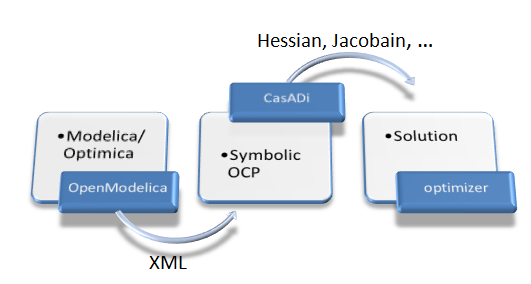
\includegraphics[width=\linewidth]{opt_tool_chain.png}
	\caption{Optimization tool chain for OpenModelica and CasADi.}
	\label{fig:optimizationtoolchain}
\end{figure}

The XML will be imported and symbolically pre-processed in CasADi. In particular, the fully-implicit DAE from
Modelica is reformulated in a semi-explicit form. With the NOCP now available in CasADi’s native data structures, the
NOCP can be reformulated to a NLP as outlined in Section \ref{sec:totalcollocations}.

At the time of writing, the efficient symbolic pre-processing model evaluation from OpenModelica is not yet completely
implemented to import into CasADi. So the symbolic preprocessing in CasADi can be used. The symbolic work in CasADi makes it easy to create the goal function \ref{eq:6} and constraints \ref{eq:7}.

The NLP is solved by one of the NLP solvers interfaced to CasADi, e.g. IPOPT \cite{wachter}. First and second order derivative information will be generated by CasADi using automatic differentiation and passed to the solver.

\section{Testing the Implementation}
\label{sec:optimizationtesting}

In this chapter, we describe the solution of an industrial-relevant optimal control problem of the diesel electric powertrain. The
formulation of the underlying optimization problem and the corresponding optimization results are presented in the
following subsections.

\subsection{Fuel optimal control of a diesel electric powertrain}
\label{sec:optimizationdiesel}

The diesel-electric powertrain model presented in \cite{sivertsson,bernhard} is a nonlinear
mean value engine model (MVEM) containing four states and three control inputs while the generator model is
simplified by considering constant efficiency and maximum power over the entire speed range, see Figure \ref{fig:dieselmodel} for the
schematic diagram of the model.

\begin{figure}
	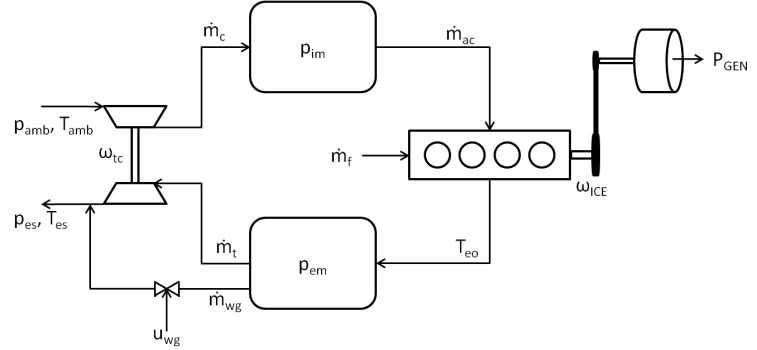
\includegraphics[width=\linewidth]{opt_diesel_model.png}
	\caption{Diagram of the diesel-electric powertrain model.}
	\label{fig:dieselmodel}
\end{figure}

In a diesel-electric powertrain the operating point of the diesel engine can be freely chosen which would potentially
decrease fuel consumption. Moreover, the electric machine has better torque characteristics. These are the main reasons
making the diesel-electric power-train concept interesting for further studies.

To investigate the fuel optimal transients of the powertrain from idling condition to a certain power level while the
accelerator pedal position is interpreted as a power level request, the following optimal control problem is solved:

\begin{equation*}
 \begin{aligned}
	\text{states}\quad x = 0, \quad \begin{pmatrix} w_{ice} \\ p_{im} \\p_{em} \\w_{tc}  \end{pmatrix}\quad = \quad \text{controls,}\quad u = \begin{pmatrix} u_{f} \\ u_{wg} \\p_{gen} \\w_{tc}  \end{pmatrix} \\
	\text{min}\;\int_{0}^{T}\dot{m}{_f} d_t
\end{aligned}
\end{equation*}

subject to

\begin{equation*}
	\begin{aligned}
		\dot{x}_1 = f_2 (x_2,x_3,u_1,u_3 ) \\
		\dot{x}_2= f_3 (x_1,x_2,x_4 ) \\
		\dot{x}_3=f_4 (x_1,x_2,x_3,u_1,u_2 ) \\
		\dot{x}_4=f_5 (x_2,x_3,x_4,u_2 ) \\
		0= f_6 (x_2,x_4 )- f_7 (x_1,x_2 ) \\
		0= f_7(x_1,x_2 ) + f_8 (x_1,u_1 )-f_9 (x_3 )-f_{10}(x_3,u_3 )  \\
		0= \frac{f_{11}(x_3)-f_{12}(x_1 )} {f_{13}(x_4 )}-f_{14} (x_4 )
\end{aligned}
\end{equation*}

\begin{equation*}
	\begin{aligned}
      54 rps \;\leq  \;  x_1  \;\leq \; 220 rps \\
      0.8 p_{amp} \;\leq \;  x_2 \; \leq \; 2P_{amb} \\
      P_{amb} \;  \leq\; x_3 \;\leq \;  3P_{amb} \\
      300rps  \; \leq \; x_4 \;\leq \;   10000 rps \\
      0 \;\leq \;u_1,u_2 \;\leq \; 1
	\end{aligned}
\end{equation*}

and boundary conditions are:

\begin{equation*}
 \begin{aligned}
	\text{at}\quad t = 0,  \begin{pmatrix} x_1 \\ x_2 \\x_3 \\x_4  \end{pmatrix} = \text{idle operating values,} \\
	\text{at}\quad t = T,  \begin{pmatrix} \dot{x}_1 \\ \dot{x}_2 \\\dot{x}_3\\\dot{x}_4 \end{pmatrix} = 0,  \begin{pmatrix} x1 \\ x2 \\x3 \\x4  \end{pmatrix} = \text{desired values} \\
	\text{and}\quad v_3 = P_{required}.
 \end{aligned}
\end{equation*}

The constraints are originated from components’ limitations and the functions $ f_i$  are described in \cite{sivertsson}.

\subsection{Model import into CasADi and NLP transcription}
\label{sec:optimizationxmlimport}

We used OpenModelica to translate Modelica/ Optimization
language extension code into an OCP in DAE and Lagrange
cost function. This OCP is then exported into an XML-based
symbolic expression format and imported into CasADi via
OpenModelica. The OCP can then be transcribed into a
nonlinear programming problem (NLP) using the approach
outlined in Section \ref{sec:totalcollocations}.

\subsection{Solution of the NLP}
\label{sec:optimizationnlp}

The NLP was solved using IPOPT \cite{wachter} running by default with the MUMPS linear solver.
The right scaling is important for a solution without oscillations.
On the other hand if the scaling does not work in all steps
then changing of the solver tolerance is helpful. The dieselmodel
is by itself well scaling in the time interval[0.32,0.5],
which is here the critical interval.

In order to cover the optimal solution of the diesel-electric
powertrain model, 140 NLP iterations for 128 sub-intervals
with the total collocation (Lobatto6 and Radau5) required by
IPOPT.

\begin{figure}
	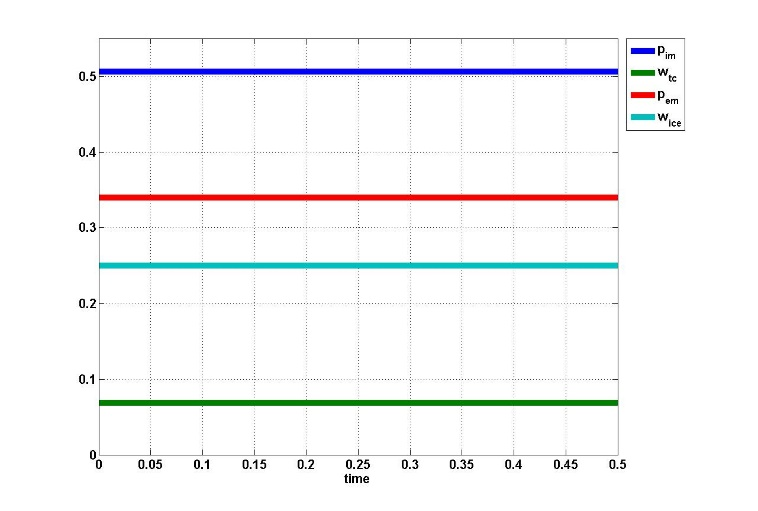
\includegraphics[width=\linewidth]{opt_initial_guess_state_variables.jpg}
	\caption{Initial guess for diesel model - state variables.}
	\label{fig:initialguessstatevariables}
\end{figure}

\begin{figure}
	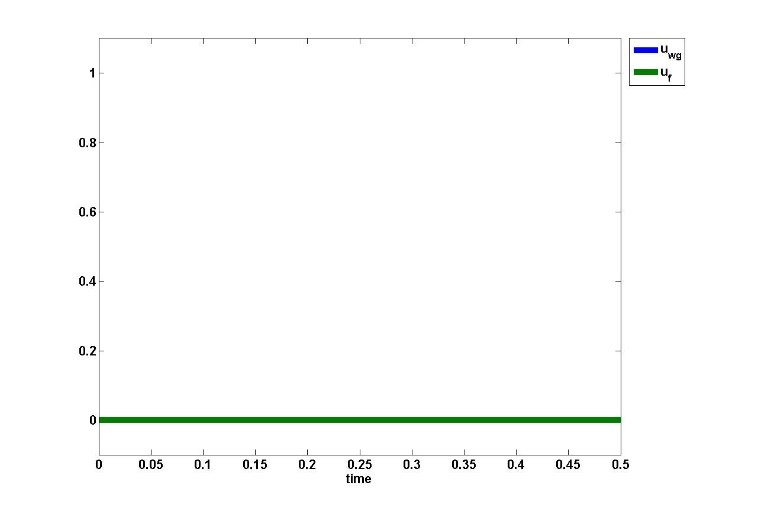
\includegraphics[width=\linewidth]{opt_initial_guess_control_variables.jpg}
	\caption{Initial guess for diesel model - control variables.}
	\label{fig:initialguesscontrolvariables}
\end{figure}


better initial guess will change the NLP iterations.
Table \ref{tab:table1} shows the total CPU time for the optimization. The calculations have been done on Dell Latitude E6410 laptop
with an Intel Core i7 processor of 2.8 GHz, 8 GB of RAM, 4M Cache, running Windows.

\begin{table}
\begin{center}
	\caption{Execution times for the diesel-electric powertrain model.} 
	\label{tab:table1} 
	\begin{tabular}{ cc } 
		\hline
		\bfseries Step & \bfseries Time  \\ 
		IPOPT (without function evaluation) & 2.140s \\ 
		NLP function evaluations & 1.158s \\ 
		\hline
	\end{tabular}
\end{center}
\end{table}

The control and state trajectories of the optimal solutions are shown in Figure \ref{fig:initialguessstatevariables} and Figure \ref{fig:initialguesscontrolvariables} respectively. The problem solved here is a minimum fuel problem for a transient 
from idle to 170 kW, for an end time of 0.5 s. For simplicity, only diesel operating condition is assumed which
means $(u_3=P_{gen} = 0)$. As it is expected, the fuel optimal results happen when engine is accelerated only near the
end of the time interval $(t\approx 0.32 s)$ to meet the end constraints while minimizing the fuel consumption.

\begin{figure}
	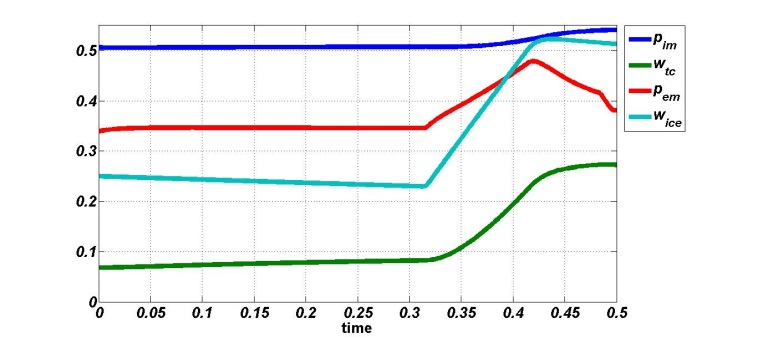
\includegraphics[width=\linewidth]{opt_result_state_variables.jpg}
	\caption{Optimization result for diesel model - state variables.}
	\label{fig:optimizationresultstatevariables}
\end{figure}

\begin{figure}
	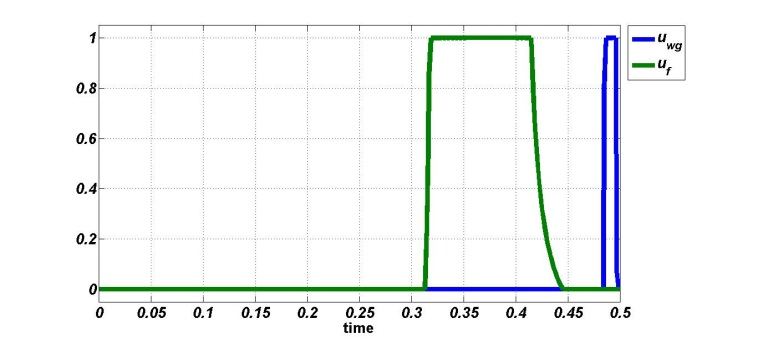
\includegraphics[width=\linewidth]{opt_result_control_variables.jpg}
	\caption{Optimization result for diesel model - control variables.}
	\label{fig:optimizationresultcontrolvariables}
\end{figure}

Amendments to the initial values, the process is robust. For this purpose, the initial values are changed slightly.

\begin{figure}
	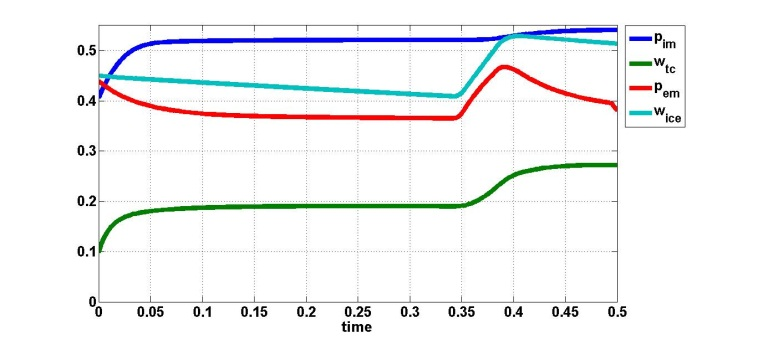
\includegraphics[width=\linewidth]{opt_result_state_variables_changed.jpg}
	\caption{Optimization result for diesel model with changed initial values - state variables.}
	\label{fig:optimizationresultchangedstatevariables}
\end{figure}

\begin{figure}
	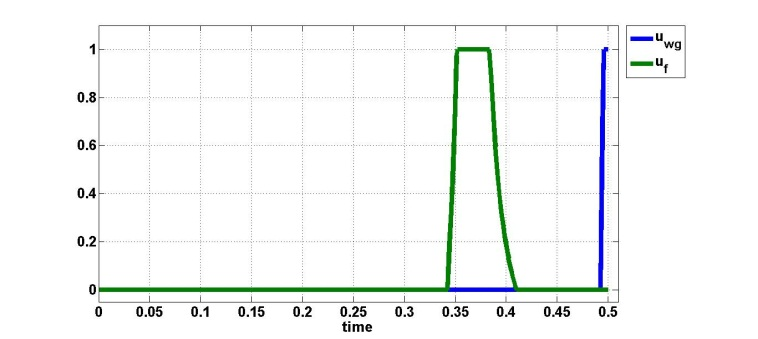
\includegraphics[width=\linewidth]{opt_result_control_variables_changed.jpg}
	\caption{Optimization result for diesel model with changed initial values - control variables.}
	\label{fig:optimizationresultchangedcontrolvariables}
\end{figure}

\subsection*{Acknowledgements}
\label{sec:optimizationacknowledgements}

This work has been partially supported by Serc, by SSF in the EDOp project and by Vinnova as well as the German
Ministry BMBF (BMBF F\"{o}rderkennzeichen: 01IS09029C) in the ITEA2 OPENPROD project and in the ITEA2 MODRIO
project. The Open Source Modelica Consortium supports the OpenModelica work.
JA and MD acknowledge support by PFV/10/002 OPTEC, GOA/10/09 and GOA/10/11, FWO G.0320.08, G.0377.09,
SBO LeCoPro; Belspo IUAP P7 DYSCO, FP7-EMBOCON (ICT-248940), SADCO (MC ITN-264735),
ERC ST HIGHWIND (259 166), Eurostars SMART, vicerp, ACCM.


%\nocite{scigen}
%We have included Paper \ref{art:scigen}

%%%%%%%%%%%%%%%%%%%%%%%%%%%%%%%%%%%%%%%%%%%%%%%%%%%%%%%%%%%%%%%%%%%%%%
%%% Intro.tex ends here


%%% Local Variables: 
%%% mode: latex
%%% TeX-master: "demothesis"
%%% End: 

%%% Intro.tex --- 
%% 
%% Filename: Intro.tex
%% Description: 
%% Author: Ola Leifler
%% Maintainer: 
%% Created: Thu Oct 14 12:54:47 2010 (CEST)
%% Version: $Id$
%% Version: 
%% Last-Updated: Thu May 19 14:12:31 2016 (+0200)
%%           By: Ola Leifler
%%     Update #: 5
%% URL: 
%% Keywords: 
%% Compatibility: 
%% 
%%%%%%%%%%%%%%%%%%%%%%%%%%%%%%%%%%%%%%%%%%%%%%%%%%%%%%%%%%%%%%%%%%%%%%
%% 
%%% Commentary: 
%% 
%% 
%% 
%%%%%%%%%%%%%%%%%%%%%%%%%%%%%%%%%%%%%%%%%%%%%%%%%%%%%%%%%%%%%%%%%%%%%%
%% 
%%% Change log:
%% 
%% 
%% RCS $Log$
%%%%%%%%%%%%%%%%%%%%%%%%%%%%%%%%%%%%%%%%%%%%%%%%%%%%%%%%%%%%%%%%%%%%%%
%% 
%%% Code:


\chapter{TLM-Based Co-Modeling Editor and Co-Simulation Framework}
\label{cha:tlm}


This chapter is based on the following paper:

\begin{itemize}
	
	
	\item  \textbf{Alachew Mengist}, Adeel Asghar, Adrian Pop, Peter Fritzson, Willi Braun, Alexander Siemers and Dag Fritzson.\textbf{ An Open-Source Graphical Composite Modeling Editor and Simulation Tool Based on FMI and TLM Co-Simulation.} In Proceedings of the 11th International Modelica Conference, Versailles, France, September 21-23, 2015. 
	
\end{itemize}

\section{Introduction}
\label{sec:tlmintroduction}

Industrial products often consist of many components which have been developed by different suppliers
using different modeling and simulation tools. An integrated modeling and simulation support is needed in order to
integrate all the parts of a complex product model. TLM-based modeling and co-simulation is an important technique for
modeling, connecting, and simulation of especially mechanical systems, which is simple, numerically stable, and efficient.
A number of tool specific simulation models, such as Modelica models, SimuLink models, Adams models, BEAST models, etc., 
have successfully been connected and simulated using TLM-based co-simulation.

This has successfully been demonstrated by integrating and connecting several different simulation
models, especially for mechanical applications. Such an integrated model consisting of several model parts
is here called a composite model since it is composed of several sub-models. Another name used for such a
model is meta-model, since it is a model of models. In earlier work \cite{tlmalexander05,tlmsiemers06}, Modelica with its object oriented modeling capabilities and its standardized graphical notations has demonstrated the possibilities for meta-modeling/composite modeling of
mechanical systems using TLM.

The availability of a general XML-based composite modeling language \cite{tlmalexander05} is an
important aspect of our TLM-based modeling and co-simulation framework. However, modelers
developing composite models are likely to take advantage of the additional availability of tools that
assist them with respect to the composite modeling process (i.e., the process of creating and/or editing a
composite model, here represented and stored as XML). 

We introduce a graphical composite model editor which is an extension and specialization of the
OpenModelica connection editor OMEdit. In the context of this work a composite
model is composed of several sub-models including the interconnections between these sub-models. 
The editor supports creating, viewing and editing a composite model both in textual and graphical representation. 
The system supports simulation of composite models consisting of sub-models created using different tools.. It is also integrated
with the SKF TLM-based cosimulation framework.

\section{TLM-Based Co-simulation Framework}
\label{sec:tlmframework}

As men\-tioned, a gen\-eral frame\-work for com\-pos\-ite model-based co-simulation has pre\-vi\-ously 
been de\-signed and im\-ple\-mented in  \cite{tlmalexander05}. The design goals for the simulation part of that framework
were portability, simplicity to incorporate additional simulation tools, and computational efficiency. 
It is also the framework used for \acrshort{tlm}-based composite model co-simulation described in this chapter.
The TLM composite model co-simulation is primarily handled by the central simulation engine of the framework 
called the \acrshort{tlm} simulation manager. It is a stand-alone program that reads an \acrshort{xml} definition
of the coupled simulation as defined in \cite{tlmalexander05}. It then starts external model simulations and
provides the communication bridge between the running simulations using the TLM \cite{tlmlakov06} method. 
The external models only communicate with the TLM simulation manager which acts as a broker and
performs communication and marshalling of information between the external models. The
simulation manager sees every external model as a black box having one or more external interfaces. The
information is then communicated between the external interfaces belonging to the different external models.
Additionally the simulation manager opens a network port for monitoring all communicated data.
TLM simulation monitor is another stand-alone program that connects to the \acrshort{tlm} simulation manager via the network port. 
The TLM simulation manager sends the co-simulation status and progress to the \acrshort{tlm}
simulation monitor via TCP/IP. The simulation monitor receives the data and writes it to an \acrshort{xml} file.

\section{Compoiste Model XML Schema}
\label{sec:tlmschema}

The composite model \acrshort{xml}-Schema for validating the co-simulation composite model is designed according
to its specification described in \cite{tlmalexander05}.The following is a sample composite model \acrshort{xml} representation:



In order to use graphical notations in the composite model editor, the composite model \acrshort{xml} file needs to describe annotations for each sub-model and connections between them. We propose to extend the composite model specification by including the \textit{Annotation}  element in the \textit{SubModel} and \textit{Connection} elements.

<Annotation Origin="{-50,54}" Extent="{-10,-10,10,10}" Rotation="0" Visible="true"/>

The contents of our composite model \acrshort{xml} root element, namely \textit{Model} is depicted in Figure \ref{fig:tlmerootelement}. Inside the root element there can be a list of connected \textit{SubModels} and TLM \textit{Connections}. \textit{SimulationParams} element is also inside the root element. It has an attribute \textit{Name} representing the name of the composite model.

\begin{figure}
	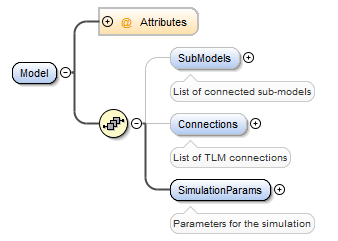
\includegraphics[width=\linewidth]{tlm_root_element.png}
	\caption{The Model (root) element of the Composite Model Schema.}
	\label{fig:tlmerootelement}
\end{figure}


The \textit{SimulationParams} element specify the start time and end time for the co-simulation.

The \textit{SubModel} element, presented in Figure \ref{fig:tlmsubmodelelement}, represents the simulation model component that participates in the co-simulation. The required attribute for a \textit{SubModel} are \textit{Name} of the sub-model, \textit{ModelFile} (file name of the submodel) and \textit{StartCommand} (the start method command to participate in the co-simulation). Each \textit{SubModel} also contains a list of interface points. \textit{InterfacePoint} elements are used to specify the \acrshort{tlm} interfaces of each simulation component (sub-model). 

\begin{figure}
	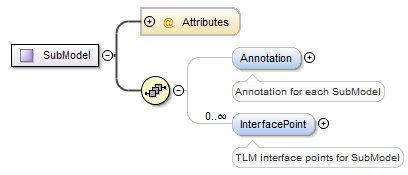
\includegraphics[width=\linewidth]{tlm_submodel_element.png}
	\caption{The SubModel element from the Composite Model Schema.}
	\label{fig:tlmsubmodelelement}
\end{figure}

The \textit{Connection} element of the composite model \acrshort{xml} schema is shown in Figure \ref{fig:tlmconnectionelement}.

\begin{figure}
	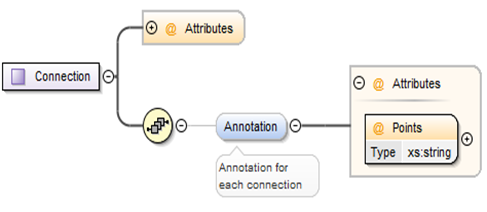
\includegraphics[width=\linewidth]{tlm_connection_element.png}
	\caption{The Connection element from the Composite Model Schema.}
	\label{fig:tlmconnectionelement}
\end{figure}

The \textit{Connection} element defines connections between two connected interface points, that is, 
a connection between two TLM interfaces. Its attributes \textit{From} and \textit{To} define which interface of which submodels are connected. Other attributes of the \textit{Connection} element specify the delay and maximum step size. 

\section{Composite Model Graphical Editor}
\label{sec:tlmeditor}

One of the primary contributions of this effort is our focus on interoperability in modeling and simulation.
Our effort leverage OpenModelica for graphical composite model editing as well as SKF’s co-simulation framework for TLM-based co-simulation. The implementation of this graphical composite model editor is an extension of OMEdit  which is implemented in C++ using the Qt graphical user interface library.

The full graphical functionality of the composite modeling process can be expressed in the following steps:

\begin{enumerate}
	
\item Import and add the external models to the composite model editor,
\item Specify startup methods and interfaces of the external model,
\item Build the composite models by connecting the external models,
\item Set the co-simulation and TLM parameters in the composite model.

\end{enumerate}

An overview of the different components that the graphical composite model editor relies on is shown in Figure \ref{fig:tlmeditorinteraction}. 

\begin{figure}
	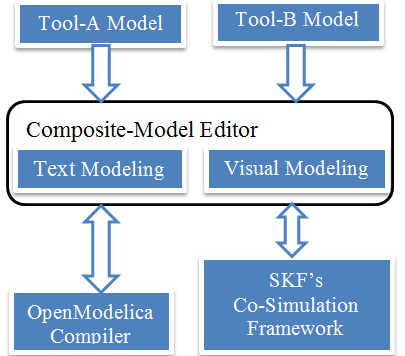
\includegraphics[width=\linewidth]{tlm_editor_interaction.png}
	\caption{An overview of the interaction between the composite model (meta-model) graphic editor and the other components.}
	\label{fig:tlmeditorinteraction}
\end{figure}

The graphical composite model editor communicates with the OpenModelica compiler to
retrieve the interface points for the external model and SKF’s co-simulation framework to run the \acrshort{tlm} simulation manager and simulation monitor. Each tool component is descried in the following subsections.

In the graphic composite model editor the modeling page area is used for visual composite modeling or text
composite modeling. This allows users to create, modify, and delete sub-models user-friendly. 

\subsection{Visual Modeling}
\label{sec:tlmvisual}

Each composite model has two views: a Text view and a Diagram view. In the diagram view, each simulation
model component (sub-model) of the \acrshort{tlm} cosimulation can be dragged and dropped from the library browser to this view, and then the sub-model will be automatically translated into a textual form by fetching the interface name for the \acrshort{tlm} based cosimulation. The user can complete the composite model (see Figure \ref{fig:tlmtest}) by graphically connecting components (sub-models).

\begin{landscape}
\begin{figure}
	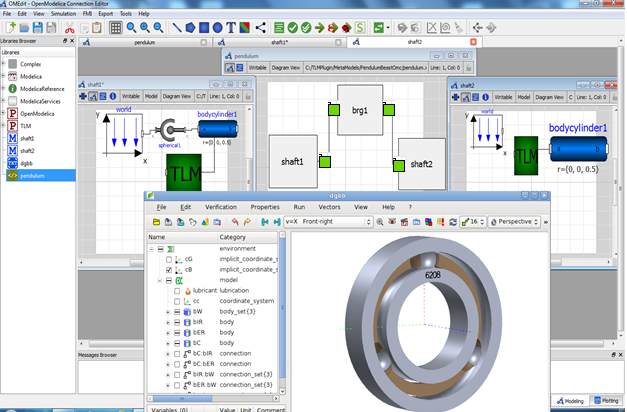
\includegraphics[width=\linewidth]{test_tlm.png}
	\caption{A screenshot of visual composite modeling of double pendulum.}
	\label{fig:tlmtest}
\end{figure}
\end{landscape}

The test model (see Figure \ref{fig:tlmtest} ) is a multibody system that consists of three sub-models: Two OpenModelica
\textit{Shaft} sub-models (\textit{Shaft1} and \textit{Shaft2}) and one SKF/BEAST bearing sub-model that together build a \textit{double pendulum}. The SKF/BEAST bearing submodel is a simplified model with only three balls to speed up the simulation. 

\textit{Shaft1} is connected with a spherical joint to the world coordinate system. The end of \textit{Shaft1} is connected via a \acrshort{tlm} interface to the outer ring of the BEAST bearing model. The inner ring of the bearing model is connected via another \acrshort{tlm} interface to \textit{Shaft2}. Together they build the double pendulum with two shafts, one spherical OpenModelica joint, and one BEAST bearing. 

\subsection{Textual Modeling and Viewing}
\label{sec:tlmtextual}

The text view (see Figure 8 \ref{fig:tlmtextview}) allows users to view the contents (sub-models, connections, and simulation
parameters) of any loaded composite model. It also enables users to edit a composite model textually as
part of the composite modeling construction process. To facilitate the process of textual composite modeling
and to provide users with a starting point, the text view (see Figure \ref{fig:tlmtextview}) includes the composite model \acrshort{xml}
schema elements and the default simulation parameters. 

\begin{landscape}
\begin{figure}
	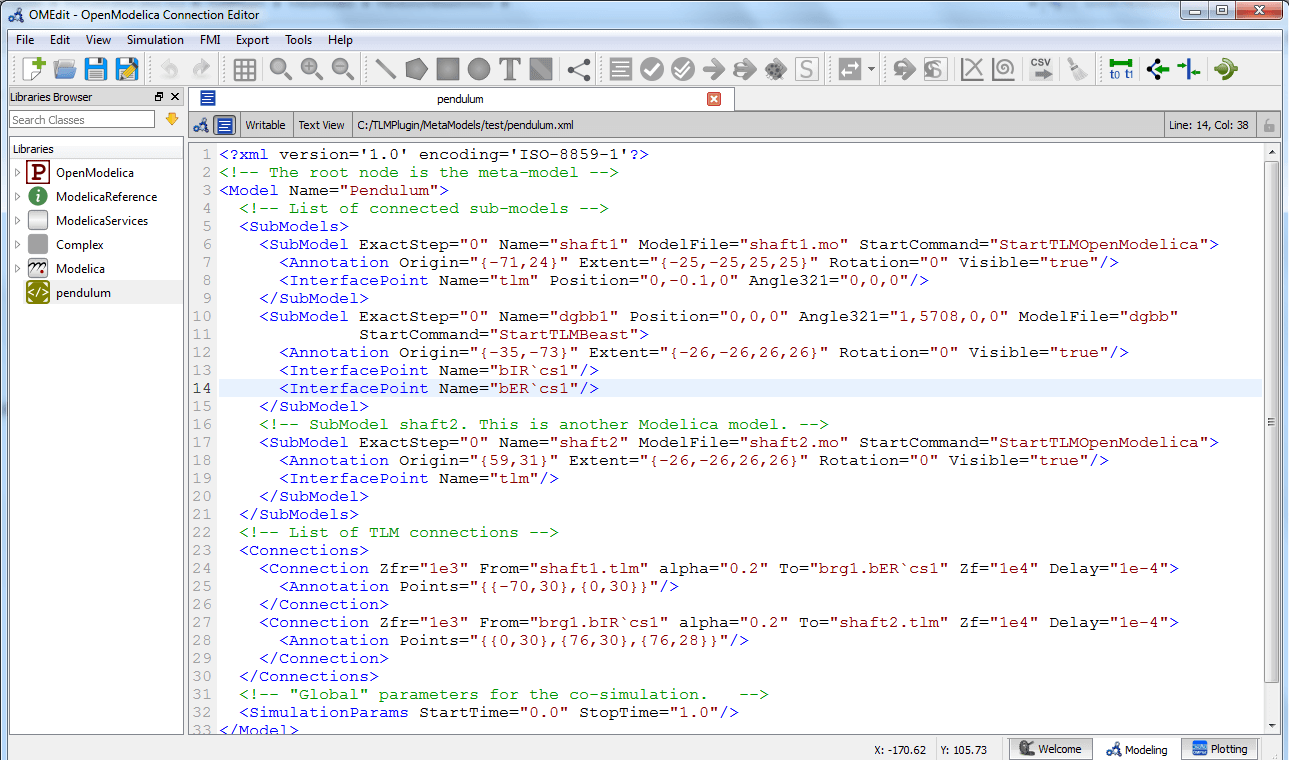
\includegraphics[width=\linewidth]{tlm_textview.png}
	\caption{A screenshot of textual composite modeling.}
	\label{fig:tlmtextview}
\end{figure}
\end{landscape}

\subsection{Composite Model Validation}
\label{sec:tlmvalidation}

Since model validation is part of the composite modeling process, the composite model editor supports users by validating the composite model to ensure that it follows the structure and content rules specified in the composite model schema described in Section 4. In general the composite model
editor validation mechanism supports users to verify that: 

\begin{itemize}

\item The basic structure of the elements and attributes in the composite model matches the composite model schema.
\item All information required by the composite model schema is present in the composite model.
\item The data conforms to the rules of the composite model schema.

\end{itemize}

\subsection{OpenModelica Runtime Enhancement}
\label{sec:tlmruntime}

To support \acrshort{tlm}-based co-simulation the OpenModelica runtime has been enhanced. The added
functionality supports single solver step simulation so that the executed simulation model can work together
with the \acrshort{tlm} manager. New flags to enable this functionality in the simulation executable are now available:

\begin{itemize}
		
\item -noEquidistantOutputFrequency
\item -noEquidistantOutputTime

\end{itemize}

The new flags control the output, e.g., the frequency of
steps and the time increment. 

\subsection{Communication with the SKF TLM Based Co-Simulation Framework}
\label{sec:tlmskf}

The graphic composite model editor in OpenModelica
provides a graphical user interface for co-simulation of
composite models. It can be launched by clicking the
\acrshort{tlm} co-simulation icon from the toolbar, see
Figure \ref{fig:tlmsetup}.

\begin{figure}
	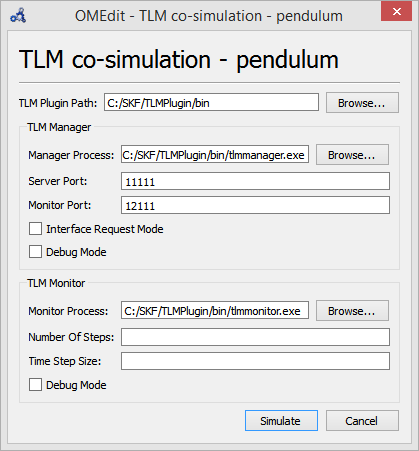
\includegraphics[width=\linewidth]{tlm_setup.png}
	\caption{TLM co-simulation setup.}
	\label{fig:tlmsetup}
\end{figure}

The editor runs the \acrshort{tlm} simulation manager and simulation monitor. The simulation manager reads the
composite model from the editor, starts the cosimulation, and provides the communication bridge
between the running simulations. Figure \ref{fig:tlmcosimulationprogress} shows the running status of the \acrshort{tlm} co-simulation.

\begin{figure}
	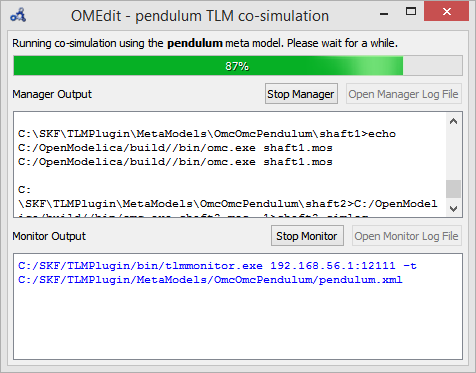
\includegraphics[width=\linewidth]{tlm_cosimulation_progress.png}
	\caption{TLM co-simulation.}
	\label{fig:tlmcosimulationprogress}
\end{figure}

The simulation monitor communicates with the simulation manager and writes the status and progress of the co-simulation in a file. This file is read by the editor for showing the co-simulation progress bar to the user. The editor also provides the means of reading the log files generated by the simulation manager and monitor.

During the post-processing stage, simulation results are collected and visualized in the OMEdit 
plotting perspective as shown in Figure \ref{fig:tlmsimulationresults}.
 
\begin{figure}
	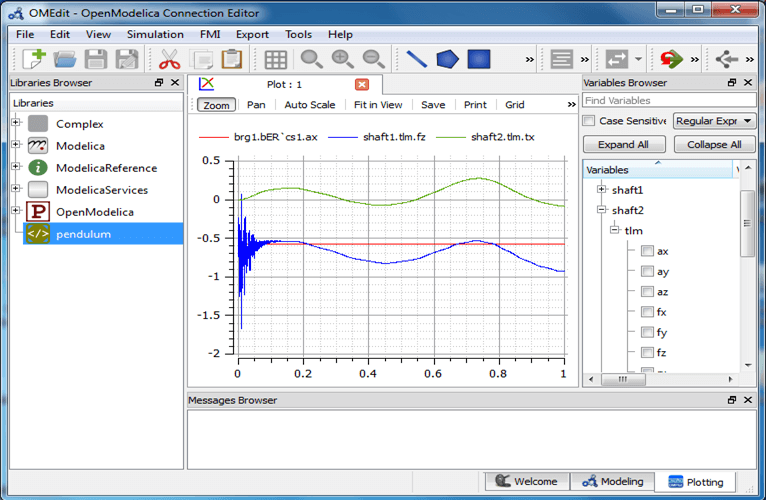
\includegraphics[width=\linewidth]{tlm_simulation_results.png}
	\caption{Results of TLM co-simulation.}
	\label{fig:tlmsimulationresults}
\end{figure}


\subsection{Industrial Application of Composite Modeling with TLM Co-Simulation}
\label{sec:tlmapplication}

SKF has successfully used the \acrshort{tlm} co-simulation framework to simulate composite models. For
example, Figure \ref{fig:tlmapplication} shows one such application with an MSC.ADAMS \cite{adams} car model
containing an integrated SKF BEAST\cite{beast} hub-unit sub-model 
connected via \acrshort{tlm}-connections.

\begin{figure}
	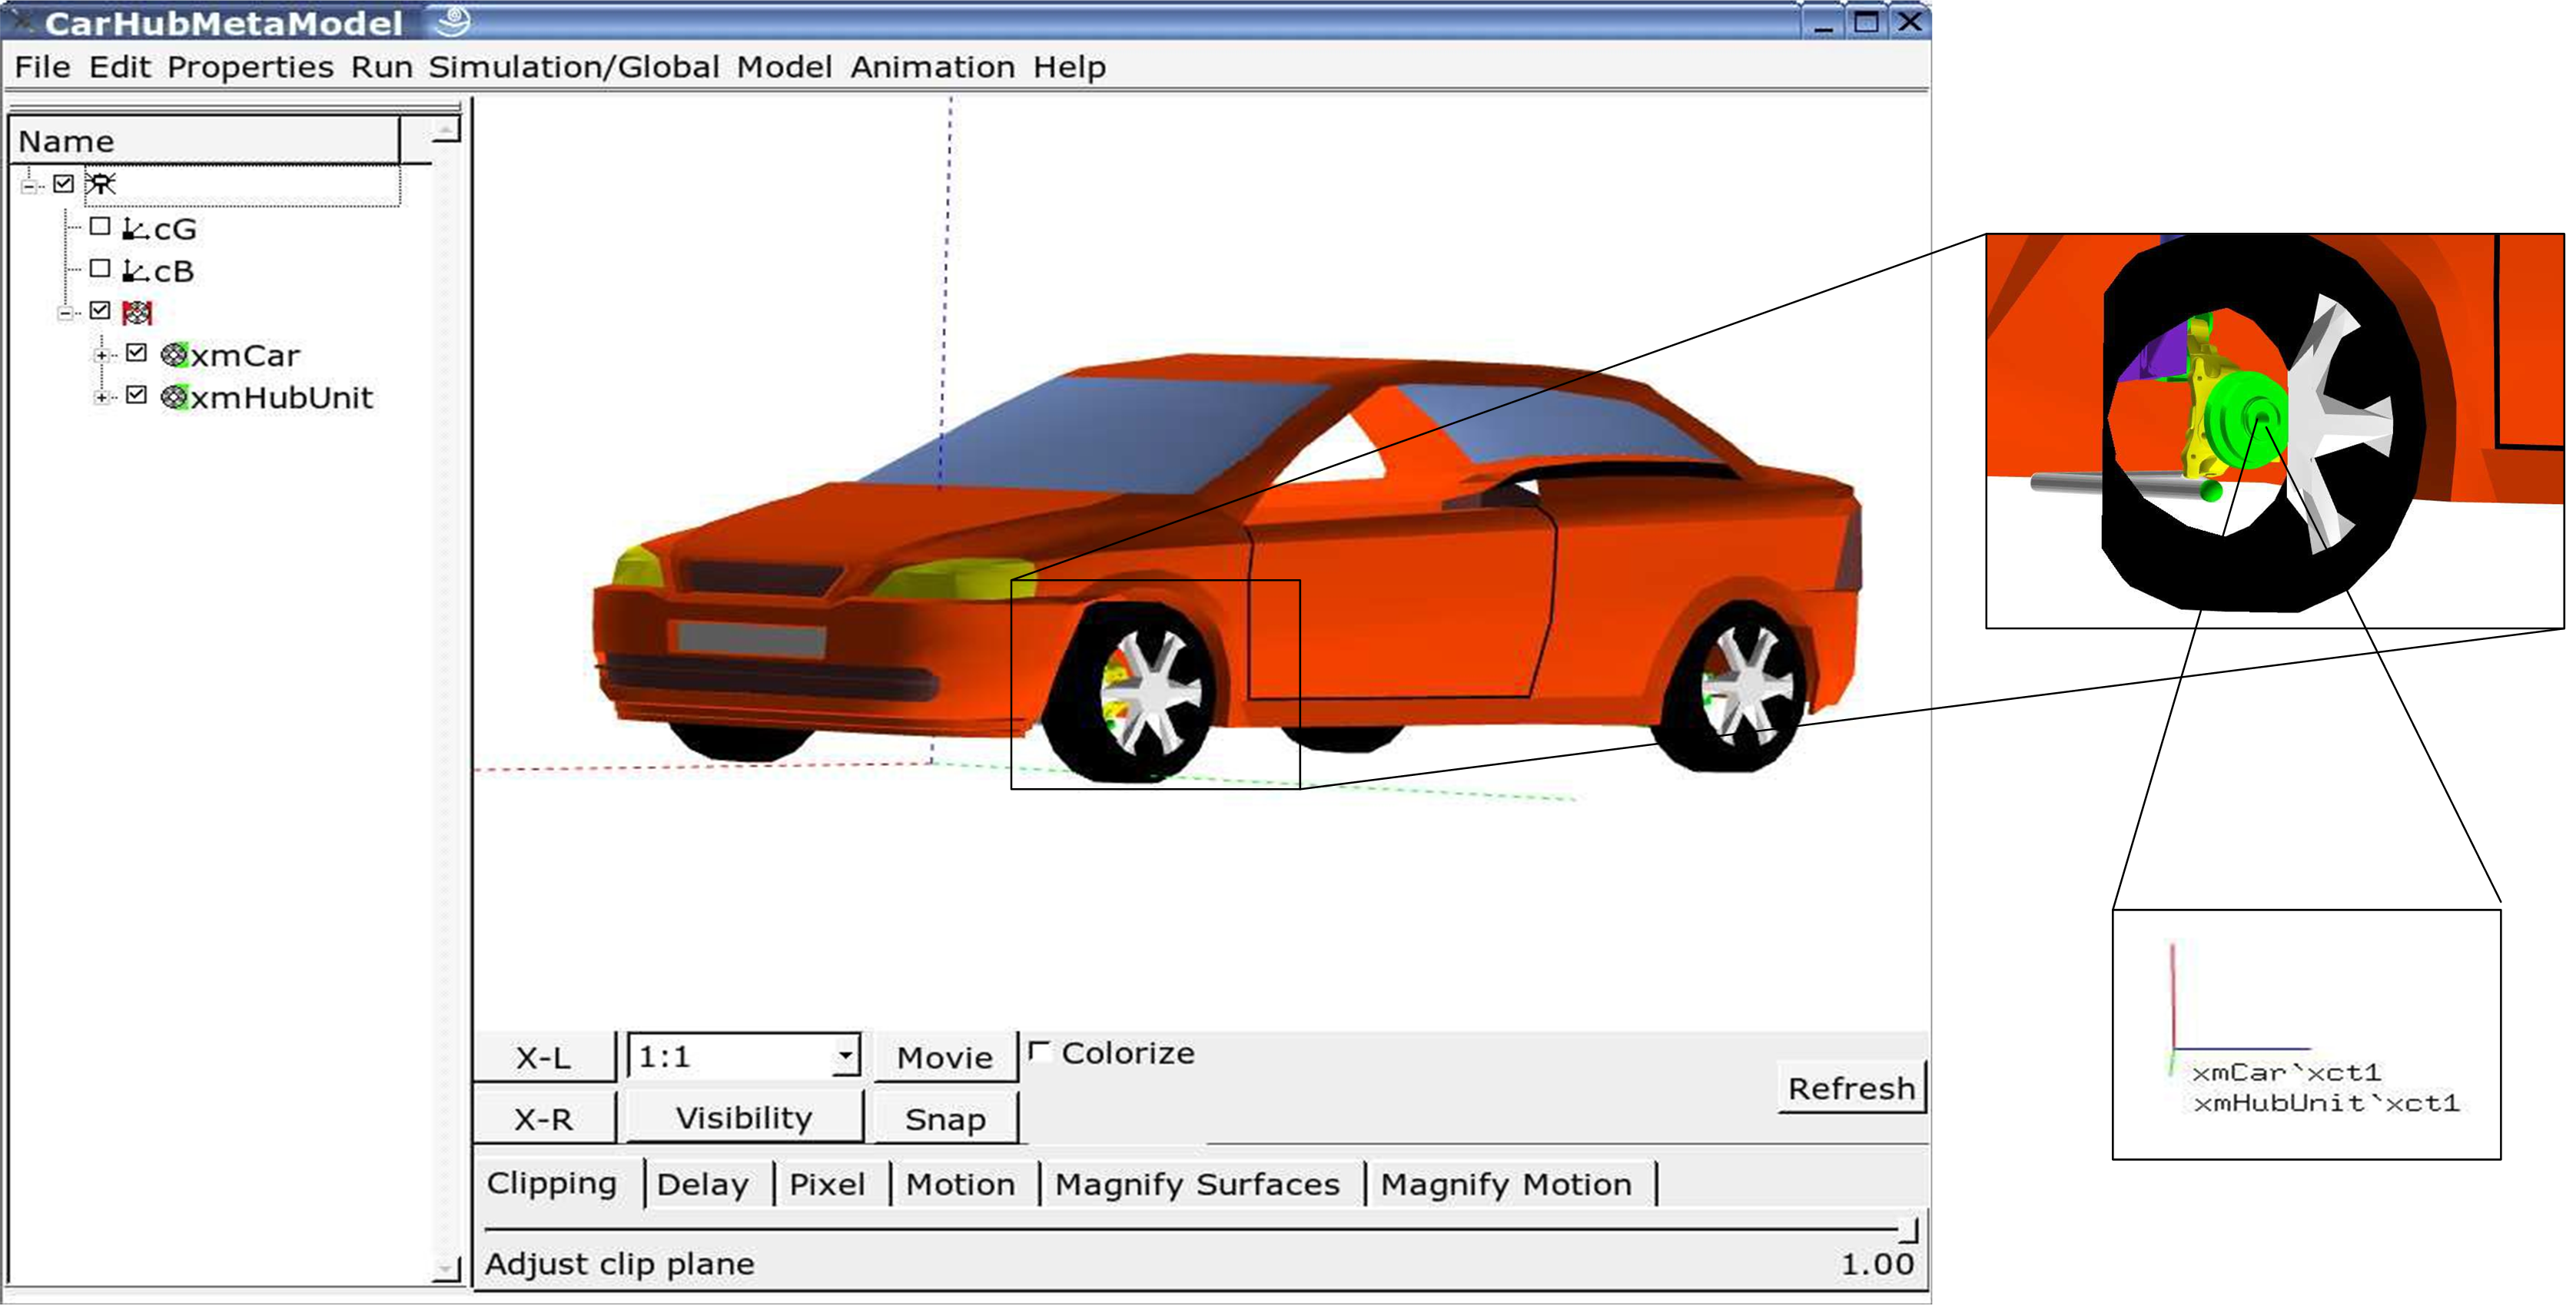
\includegraphics[width=\linewidth]{tlm_application.png}
	\caption{A composite model of an MSC.ADAMS car model with an integrated SKF BEAST hub-unit sub-model (green), connected 
		     via TLM connections for co-simulation.}
	\label{fig:tlmapplication}
\end{figure}

\section{Summary}
\label{sec:tlmsummary}

In this chapter, we introduced a general open-source graphical editor and simulation tool for composite modeling and co-simulation as well as its integration with SKF’s TLM-based co-simulation framework for TLM based co-simulation. The graphical editor combines a number of features to support end-users with respect to the creation of composite models and co-simulation. These include adding, removing, and connecting components (submodels) both textually and graphically, as well as integrated co-simulation and visualization of simulation results. The composite model editor supports external non-Modelica models represented in XML form (essentially black boxes with interfaces) inside the component tree which can be used for composite model composition. A number of tool specific simulation models, such as Modelica models, SimuLink models, Adams models, BEAST models,
etc., have successfully been connected and simulated using TLM based co-simulation. A schema for validation of a composite modeling has been developed as a part of this work. 

\subsection*{Acknowledgements}
\label{sec:tlmAcknowledgements}

The work has been supported by Vinnova in the ITEA2
MODRIO project, by EU in the INTO-CPS project, and by the Swedish Government in the Swedish
Government in the ELLIIT project. The open-source Modelica Consortium supports the OpenModelica
work. The TLM based co-simulation framework is provided by SKF.


%\nocite{scigen}
%We have included Paper \ref{art:scigen}

%%%%%%%%%%%%%%%%%%%%%%%%%%%%%%%%%%%%%%%%%%%%%%%%%%%%%%%%%%%%%%%%%%%%%%
%%% Intro.tex ends here


%%% Local Variables: 
%%% mode: latex
%%% TeX-master: "demothesis"
%%% End: 

%%% Intro.tex --- 
%% 
%% Filename: Intro.tex
%% Description: 
%% Author: Ola Leifler
%% Maintainer: 
%% Created: Thu Oct 14 12:54:47 2010 (CEST)
%% Version: $Id$
%% Version: 
%% Last-Updated: Thu May 19 14:12:31 2016 (+0200)
%%           By: Ola Leifler
%%     Update #: 5
%% URL: 
%% Keywords: 
%% Compatibility: 
%% 
%%%%%%%%%%%%%%%%%%%%%%%%%%%%%%%%%%%%%%%%%%%%%%%%%%%%%%%%%%%%%%%%%%%%%%
%% 
%%% Commentary: 
%% 
%% 
%% 
%%%%%%%%%%%%%%%%%%%%%%%%%%%%%%%%%%%%%%%%%%%%%%%%%%%%%%%%%%%%%%%%%%%%%%
%% 
%%% Change log:
%% 
%% 
%% RCS $Log$
%%%%%%%%%%%%%%%%%%%%%%%%%%%%%%%%%%%%%%%%%%%%%%%%%%%%%%%%%%%%%%%%%%%%%%
%% 
%%% Code:


\chapter{Collaborative Modeling and Traceability of CPSs}
\label{cha:traceability}


\section{Introduction}
\label{sec:tracaebilityintroduction}


Modeling and simulation tools have become increasingly used for industrial applications. Such tools support different 
activities in the modeling and simulation lifecycle,like specifying requirements, model creation, model simulation, \acrshort{fmu} 
export, model checking, and code generation. However, the heterogeneity and complexity of modern industrial products often require special purpose modeling and simulation tools for different phases of the development life cycle. Seamless exchange of models between different modeling tools
is needed in order to integrate all the parts of a complex product model throughout the development life cycle. 

During the past decade, the \acrshort{oslc} specifications\cite{oslc} 
have emerged for integrating development lifecycle tools using Linked Data \cite{linkeddatatom,linkeddata,linkeddatatim}. For traceability purposes, in particular the \acrshort{oslc} Change Management specification is relevant. In earlier work \cite{oslcelaasar} \acrshort{oslc} has successfully been demonstrated for integration of modeling tools in general, and traceability in particular. 

In the previous version of OpenModelica \cite{debugingpop} the compiler supports traceability in terms of tracing 
generated C code back to the originating Modelica source code, but not in the \acrshort{oslc} sense, and mostly used for debugging. 

In this chapter we present new traceability support in OpenModelica where the traceability information is exchanged with other lifecycle 
tools through a standardized interface and format using \acrshort{oslc}. In particular, OpenModelica supports automatic recording and tracing of
modeling activities such as creation, modification, and destruction of models, import of model description \acrshort{xml}, export of FMUs, and creation of simulation results to link models from various tools. OpenModelica supports simple queries (traces to and traces from) to present the traceability information to the user.


\section{Open Services for Lifecycle Collaboration (OSLC)}
\label{sec:tracaebilityoslc}

Open Services for Lifecycle Collaboration (OSLC) \cite{oslc} is an open source initiative
for creating a set of specifications that enables integration of development life cycle tools (e.g.,
modeling tools, change management tools, requirements management tools, quality management
tools, configuration management tools). The goal of \acrshort{oslc} is to make it easier for tools to work together by
specifying a minimum amount of protocol without standardizing the behavior of a specific tool.

The \acrshort{oslc} specifications use the Linked Data model to enable integration at the data level via links between
tool artifacts defined as Resource Description Framework (RDF) \cite{rdffrank} resources (beside other possible representations such as
\acrshort{xml}, JavaScript Object Notation (JSON) \cite{json}, Atom, and Turtle). The resources are identified
by HTTP URIs. A common protocol to perform creation (HTTP POST) and retrieval (HTTP GET), update (HTTP PUT) and delete (HTTP DELETE) operations on resources is also specified.


\section{Traceability Design and Architecture}
\label{sec:tracaebilitydesign}


The traceability design and architecture is mainly being developed in the INTO-CPS project \cite{intocpspaper,intocps} 
which contains a set of tasks. One of these is the design of traceability and model management with the following goals (Lausdahl et al, 2016):

\begin{itemize}
\item Checking the realization of requirements in models
\item Enabling collaborative work by connecting artifacts and knowledge from different users
\item Decreasing redundancy by connecting different tools to a single requirements source and allowing
a system-wide view that is not only limited to single tools
\end{itemize}

The Provenance (PROV) \cite{provluc} and \acrshort{oslc} standards presented in \cite{intocpsjohn})
are used to support traceability activities. PROV is a set of documents built on the notation and relation of
entities, activities, and agents.

The design and architecture of the traceabilityrelated tools has recently been developed in \cite{intocpskenneth} and is shown in Figure  \ref{fig:traceabilityarchitecture}. Any modeling tool written in any programming language can use these traceability standards to support the traceability of activities performed within the tool and interact with other tools.

\begin{figure}
	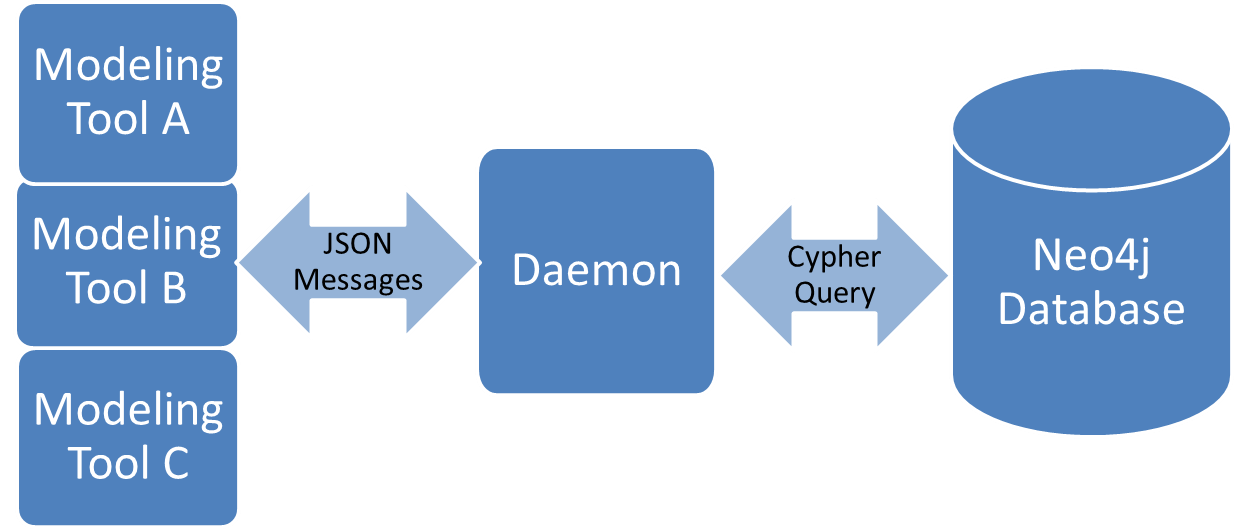
\includegraphics[width=\linewidth]{traceability_architecture.png}
	\caption{Schematic architecture of the traceability related tools.}
	\label{fig:traceabilityarchitecture}
\end{figure}


As depicted in Figure 1 \ref{fig:traceabilityarchitecture}, the architecture is divided into three parts:

\begin{description}
\item[Modeling Tools] The modeling tools send traceability information from activities that are performed within the tools (e.g., model creation,
modification, import model description in \acrshort{xml}) to the daemon.
\item[Daemon] The daemon provides an \acrshort{oslc} interface compliant with RESTful \cite{restfulleonardo} to store the traceability 
information into the database and retrieve the traceability data from the database. It is launched and terminated by modeling tools.
\item[Neo4j Graph Database] The Neo4j database \cite{neo4j} is a graph database to store the \acrshort{oslc} triples that make up the traceability data. 

\end{description}

\section{An Example of Integrated Tools for Cyber-Physical Model Development}
\label{sec:tracaebilitytools}

OpenModelica has been successfully integrated with the INTO-CPS tool chain to trace artifacts created
during the system development process from high level requirements to simulation results. The tools involved
are Overture (Larsen et al, 2010), 20-sim (Controllab Products B.V, 2013), Modelio (Favre, 2005) and RTTester
(Verified Systems International GmbH, 2012). The tool chain as shown in Figure \ref{fig:traceabilitytools} is defined by the
connections between the system architecture and the simulation via the model description \acrshort{xml} file and the \acrshort{fmu}.

\begin{figure}
	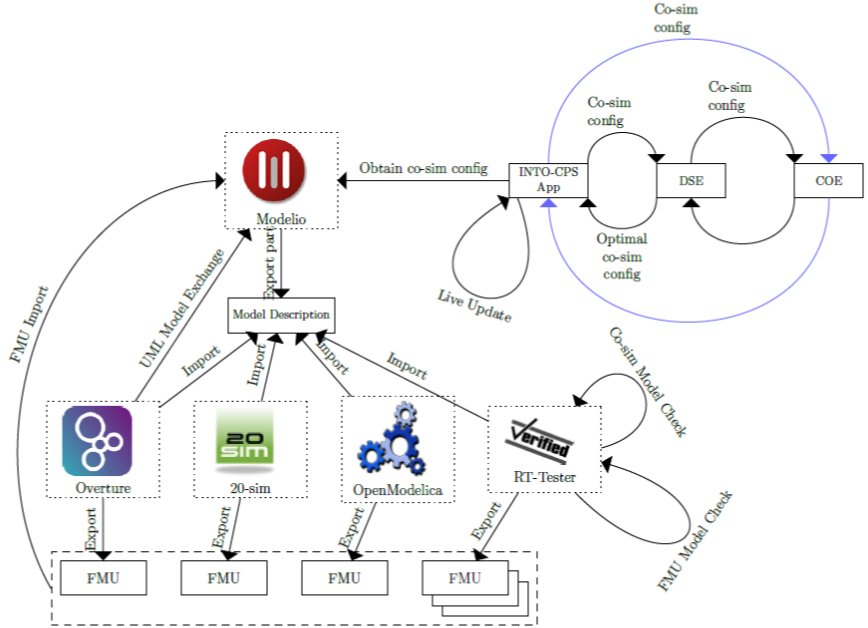
\includegraphics[width=\linewidth]{traceability_tools.png}
	\caption{An Example of integrated tools to trace artifacts created during the system development process (Bandur et al, 2016).}
	\label{fig:traceabilitytools}
\end{figure}

The \acrshort{sysml} Connection diagram defines the components of the system and their connections. The
internals of these block instances are created in the various modeling tools and exported as FMUs. 
The modeling tools support importing the interface definition (ports) of the blocks in the Connection
diagram by importing a modelDescription.xml file containing the block name and its interface definition
linked with requirements. All tools are storing information in Git and sending information about
existing and created artifacts to the global database.

\section{Traceability and Model Management in OpenModelica}
\label{sec:tracaebilityactivities}

In the new work reported in this chapter, OpenModelica has been extended with support of traceability in the \acrshort{oslc} sense, 
where traceability information is exchanged with external tools through a standardized interface and format. The implementation is based on
an architecture and a common interface defined in \cite{intocpskenneth} for exchanging traceability information. 

The modeling activities that can be recorded automatically and traced within OpenModelica are:

\begin{itemize}
\item Model description \acrshort{xml} import (linked with requirements)
\item Model creation
\item Model modification
\item Model destruction
\item FMU export
\item Simulation result creation

\end{itemize}
The complete workflow for traceability artefacts within OpenModelica and the different components that rely on are shown in Figure \ref{fig:traceabilityworkflow}.

The following summarizes the main workflow that could be used to create and record traceability
information in OpenModelica during cyber-physical model development process.

\begin{enumerate}
\item Commit model file entity to Git repository and record the Git-hash
\item Create URIs of the activity based on the Git\-hash
\item \acrshort{oslc} triples describing the activity are generated using the URIs
\item \acrshort{oslc} triples are sent to the traceability Daemon
\item Retrieve the traceability information (traces to and traces from)

\end{enumerate}

The traceability information is represented in \acrshort{json} format. The modeling activities described by \acrshort{oslc}
triples represented in \acrshort{json} format are sent from OpenModelica to the daemon. These traces are then
sent through the daemon to the Neo4j database, where they are stored. In order to view and analyze
traceability data, this is later retrieved (traces to and traces from) from OpenModelica, through the
appropriate queries from the daemon to the database. 

\begin{figure}
	\includegraphics[width=\linewidth]{traceability_workflow.png}
	\caption{Workflow of traceability of artifacts during the system development process in OpenModelica.}
	\label{fig:traceabilityworkflow}
\end{figure}



\section{Prototype Implementation}
\label{sec:tracaebilityprototype}

We have implemented a prototype to demonstrate the idea of exchanging traceability information for
integrating lifecycle modeling tools using \acrshort{oslc}. The prototype is implemented based upon the design and
architecture presented in Section \ref{fig:traceabilityarchitecture}.

As mentioned, the implementation of this prototype is an extension of OMEdit (Asghar et al, 2010) which
is implemented in C++ using the Qt Framework (Nokia Corporation, 2011) graphical user interface library. For
presentation reasons, we have grouped the prototype functionality into three categories: importing model
description XML, model management with Git integration, and traceability support using \acrshort{oslc}, 
which are described in the following subsections.


\subsection{Import Model Description in XML}
\label{ssec:tracaebilityimprtxml}

As a preparation for the extension to support tracing for importing modelDescription.xml interface files, we 
extended OpenModelica to support importing modelDescription.xml (See Figure \ref{fig:traceabilityimportfmu}) . 

\begin{figure}
	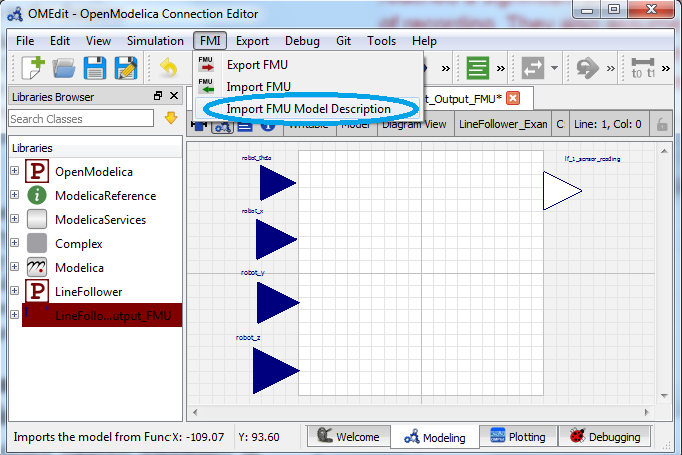
\includegraphics[width=\linewidth]{traceability_import_fmu.png}
	\caption{A screen shot of the model description XML import operation.}
	\label{fig:traceabilityimportfmu}
\end{figure}

OpenModelica can import model description \acrshort{xml} interface files (linked with requirements) created using
other system architectural modeling tools and create  Modelica models from this information. The result is a
generated file with a Modelica model stub containing the inputs and outputs specified in the model
Description.xml file. Then the user can create a complete model using the GUI via drag and drop in the
editor. Hence, the traceability chain within OpenModelica traces models linked with requirements
through model description \acrshort{xml} import, model creation, model modification, \acrshort{fmu} export and simulation results.

\subsection{Model Management with Git Integration}
\label{sec:tracaebilitygit}

One of the objectives of the traceability tooling is to manage the development process in terms of modeling
activities within the modeling tools. In order to achieve this objective access to the version control system is
required in OpenModelica. Therefore the OpenModelica Connection Editor OMEdit has been enhanced to support Git version 
control as shown in Figure \ref{fig:traceabilitygit}.

\begin{figure}
	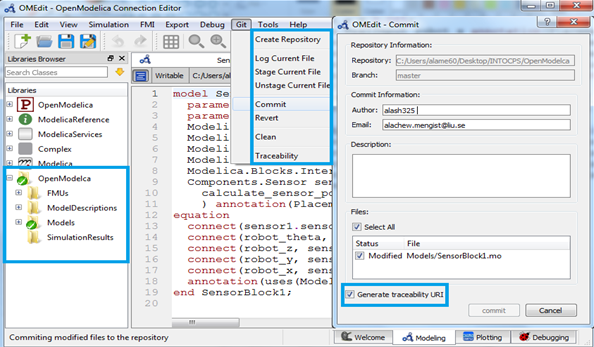
\includegraphics[width=\linewidth]{traceability_git.png}
	\caption{GUI of Git Integration in OpenModelica and functions available to create traceability URI.}
	\label{fig:traceabilitygit}
\end{figure}

The OMEdit Git integration is currently in an early stage of development but already supports some basic
functionality (See Figure \ref{fig:traceabilitygit}) such as staging modified tracing operations on files 
for commit, committing, and reverting changes. It is useful to provide viewing of status and version history 
which can be used for creating the resource URIs for the modeling activities on each new commit.

The implemented prototype also allows to create a local Git repository by selecting Git -> Create New Repository from the menu bar. 
Since the URI, as presented in \cite{intocpsjohn} is the combination of the Git-hash and the unique path for every file in the
project, creating a Git repository for traceability purposes automatically adds a structure (See the left
part of Figure \ref{fig:traceabilitygit}) for models, simulation results, FMUs, and model description \acrshort{xml} files to the Git repository.

\subsection{Traceability Support in OpenModelica}
\label{ssec:traceabilityopenmodelica}

The traceability support in OpenModelica provides a graphical user interface to interact with other lifecycle
modeling tools.

As already mentioned in Section 4 [***], OpenModelica supports traceability in the \acrshort{oslc} sense, where
traceability information is exchanged with external tools through a standardized interface and format. 
The implementation is based on the architecture and a common interface defined in \cite{intocpskenneth} for 
exchanging traceability information. OpenModelica imports the modelDescription.xml and creates a Modelica model according to the \acrshort{fmu}
interface. The generated Modelica model is completed with behavior for the \acrshort{sysml} block and the final model
is exported in the \acrshort{fmu} form. The generated \acrshort{fmu} is then used in a whole system simulation connected
according to the \acrshort{sysml} connection diagram. The \acrshort{fmu} master simulation algorithm component performs
the simulation via the INTO-CPS App. This whole chain is traced using \acrshort{oslc}.

We have designed a graphical user interface shown in Figure 6 [***] which allows the user to record the
traceability information and send to the Daemon (\acrshort{oslc} triples in \acrshort{json} format), describing the activity
using the URIs generated in the GUI shown in Figure 5[****]. The PROV and \acrshort{oslc} relations that are mainly used
in this work can be found in \cite{intocpsjohn}.
  
These traces are then sent through the daemon to the database via HTTP POST http://localhost:8080/
traces/push/json, where they are stored. Figure \ref{fig:traceabilitygraph} shows an example of traceability information 
sent from OpenModelica to the daemon and visualized in the Neo4j database.
\begin{landscape}
\begin{figure}
	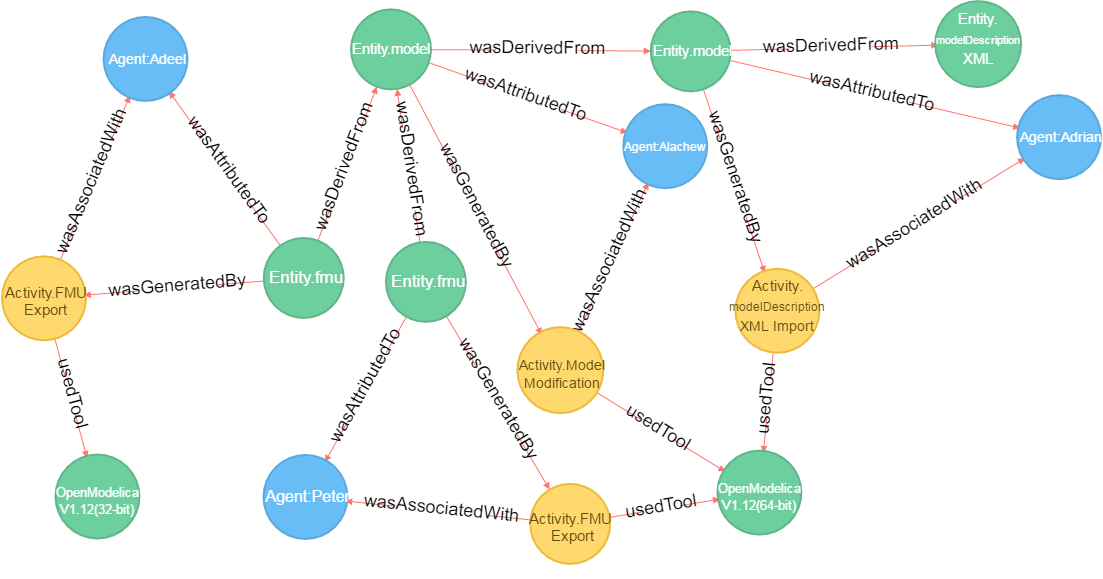
\includegraphics[width=\linewidth]{traceability_graph.png}
	\caption{An example of traceability information sent from OpenModelica to the daemon and visualized in the Neo4j database.}
	\label{fig:traceabilitygraph}
\end{figure}
\end{landscape}

Entities (e.g. Modelica files, FMUs,modelDescription XML file) are shown in green,
actions (e.g. model creation, FMU export, modelDescription XML import) are shown in yellow,
agents (e.g. users with the names {"Alachew"}, {"Adrian"}, {"Peter"}, and {"Adeel")} are shown in blue,
and their relationships \"what come from what\" and \"what used what\" (e.g. \"wasGeneratedBy\", \"wasDerivedFrom\", \"usedTool\") are 
shown with red arrows.

In order to view and analyze traceability data, we have also designed a graphical user interface shown in
Figure 8 [***] which allows the user to query traceability information (traces to and traces from) from the
daemon to the database (via HTTP GET):

\begin{itemize}
\item http://localhost:8080/traces/from/<URI>/json and
\item http://localhost:8080/traces/to/<URI>/json 

\end{itemize}
 
\section{Summary and Discussion}
\label{sec:traceabilitysummary}


\subsection*{Acknowledgments}
\label{sec:traceabilityacknowledgments}

This work has been supported by the European Union in the H2020 INTO-CPS project. Support from
Vinnova in the ITEA3 OPENCPS project has been received. The OpenModelica development is supported
by the Open Source Modelica Consortium. Special thanks to Kenneth Lausdahl, Peter Niermann, Jos H\"{o}ll,
Carl Gamble, Oliver M\"{o}ller, Etienne Brosse, Tom Bokhove, and Luis Diogo Couto for collaboration and
valuable input to traceability related tools design.


%\nocite{scigen}
%We have included Paper \ref{art:scigen}

%%%%%%%%%%%%%%%%%%%%%%%%%%%%%%%%%%%%%%%%%%%%%%%%%%%%%%%%%%%%%%%%%%%%%%
%%% Intro.tex ends here


%%% Local Variables: 
%%% mode: latex
%%% TeX-master: "demothesis"
%%% End: 

%%% Intro.tex --- 
%% 
%% Filename: Intro.tex
%% Description: 
%% Author: Ola Leifler
%% Maintainer: 
%% Created: Thu Oct 14 12:54:47 2010 (CEST)
%% Version: $Id$
%% Version: 
%% Last-Updated: Thu May 19 14:12:31 2016 (+0200)
%%           By: Ola Leifler
%%     Update #: 5
%% URL: 
%% Keywords: 
%% Compatibility: 
%% 
%%%%%%%%%%%%%%%%%%%%%%%%%%%%%%%%%%%%%%%%%%%%%%%%%%%%%%%%%%%%%%%%%%%%%%
%% 
%%% Commentary: 
%% 
%% 
%% 
%%%%%%%%%%%%%%%%%%%%%%%%%%%%%%%%%%%%%%%%%%%%%%%%%%%%%%%%%%%%%%%%%%%%%%
%% 
%%% Change log:
%% Completed Language Reading MBS
%% 
%% RCS $Log$
%%%%%%%%%%%%%%%%%%%%%%%%%%%%%%%%%%%%%%%%%%%%%%%%%%%%%%%%%%%%%%%%%%%%%%
%% 
%%% Code:


\chapter{Advanced Modeling Simulation Analysis}
\label{cha:python}


This chapter is based on the following papers:

\begin{itemize}
		
	\item Bernt Lie, Sudeep Bajracharya, \textbf{Alachew Mengist}, Lena Buffoni, Arun Kumar, Martin Sj\"{o}lund, Adeel Asghar, Adrian Pop, Peter Fritzson.\textbf{ API for Accessing OpenModelica Models From Python.} In Proceedings of 9th EUROSIM Congress on Modeling and Simulation, September 12-16, 2016, Oulu, Finland. 
	
	\item Adeel Asghar, Andreas Pfeiffer, Arunkumar Palanisamy, \textbf{Alachew Mengist}, Martin Sj\"{o}lund, Adrian Pop and Peter Fritzson.\textbf{ Automatic Regression Testing of Simulation Models and Concept for Simulation of Connected FMUs in PySimulator.} In Proceedings of the 11th International Modelica Conference, Versailles, France, September 21-23, 2015. 
		
\end{itemize}

\section{Introduction}
\label{sec:pythonintroduction}

EOO languages such as Modelica have relatively little support for the advanced model analysis and synthesis needed for control systems design, particularly for optimal control problems (OCPs). Examples of such desirable analysis capabilities include (i) study of model sensitivity, (ii) random number generation and statistical analysis, (iii) Monte Carlo simulation, (iv) advanced plotting capabilities, (v) general optimization capabilities, (vi) linear analysis and control synthesis, etc. Scripting languages such as MATLAB and Python include most of these desirable analytical capabilities, and it is of interest to integrate Modelica models with such scripting languages. For the purposes of this work, we have chosen to use Python and OpenModelica due to their open-source availability.

A Python API for controlling Modelica simulation and analysis from Python was proposed in February 2015\footnote{Python API for Accessing OpenModelica Models, by B. Lie, February 20, 2015.}. Based on this proposal, we have developed an initial version of a Python API for operating on Modelica models in Python. In this chapter, we present how to generate a Python object from an EOO Modelica model, how to set operating conditions, and how to run the simulation to produce a result object. Furthermore, we describe how to carry out linearization of a model object, the possibility of carrying out parameter sensitivity studies, and how to extract results from the result object to Python. The proposed solution has been tested on several industrially-relevant models, and its use for automatic analysis of Modelica models from Python is illustrated using a simple water tank model.

\section{Description of the API}
\label{sec:pythonapi}

The API is described in the subsections below.

\subsection{Python Class and Constructor}
\label{subsec:pythonclass}

The name of the Python class that is used for operation on Modelica models is \textit{ModelicaSystem}.
This \textit{class} is equipped with an object constructor with the same name as the class. In addition, the class is equipped
with a number of methods for manipulating the instantiated objects. In this subsection, we discuss how to import the class, and
how to use the constructor to instantiate an object. The object is imported from package OMPython, i.e., with
Python commands.

\begin{lstlisting}
  >>>from OMPython import ModelicaSystem
\end{lstlisting}

Other Python packages to be used, such as \textit{numpy},\textit{matplotlib}, \textit{pandas}, etc. must be imported in a similar
manner. The object constructor requires a minimum of 2 input arguments which are strings, and may need a third string input
argument.

\begin{itemize}
	\item The \textit{first input argument} must be a string with the file name of the Modelica code, with Modelica file extension\textit{.mo}. If the 	 
	       Modelica file is not in the current directory of Python, then the file path must also be included.
	\item The \textit{second input argument} must be a string with the name of the Modelica model, including the namespace if the model is wrapped 
		  within a Modelica package.
	\item A \textit{third input argument} is used if the Modelica model builds on other Modelica code, e.g., the Modelica Standard Library.
\end{itemize}

Example 1: Use of constructor. Suppose we have a Modelica model with name CSTR wrapped in a Modelica package \textit{Reactors} — stored in file
\textit{Reactor.mo}:

\begin{lstlisting}
package Reactors
	// ...
	model CSTR
		/// ...
	end CSTR;
	//
end Reactors;
\end{lstlisting}

If this model does not use any external Modelica code and the file is located in the current Python directory, the following
Python code instantiates a Python object \textit{mod}:

\begin{lstlisting}
>>> mod = ModelicaSystem('Reactors.mo','Reactors.CSTR')
\end{lstlisting}

The user is free to choose any valid Python label name for the Python object. All methods of class \textit{ModelicaSystem} refers to the instantiated object, in standard Python fashion. Thus, method \textit{simulate()} is invoked with the Python command:

\begin{lstlisting}
>>>mod.simulate()
\end{lstlisting}

In the subsequent overview of methods, the object name is not included. In practice, of course, it must be included in order
to operate on the object in question. Methods may have no input arguments, one, or several input arguments. Methods may or may not return results — if the methods do not return results, the results are stored within the object.

\subsection{Utility routines, converting Modelica $\leftrightarrow$ FMU:}
\label{subsec:pythonmodelicafmu}
Two utility methods convert files between Modelica files with file extension \textit{.mo} and Functional Mock-up Unit (FMU) files with
file extension \textit{.fmu}.

\begin{enumerate}
	\item \textit{convertMo2Fmu()} — method for converting the Modelica model of the object, say ModelName, into FMU file.
	\begin{itemize}
		\item Required input arguments: none, operates on the Modelica file associated with the object.
		\item Optional input arguments:
		\begin{itemize}
			\item \textit{className}: string with the class name that should be translated,
			\item \textit{version}: string with FMU version, "1.0" or "2.0"; the default is "1.0".
			\item \textit{fmuType}: fmuType: string with FMU type, "me" (model exchange) or "cs" (co-simulation); the default is "me".
			\item \textit{fileNamePrefix}: string; the default is \'className\'.
			\item \textit{generatedFileName}: string, returns the full path of the generated FMU.
		\end{itemize}
		\item Result: file \textit{ModelName.fmu} in the current directory
	\end{itemize}
	\item \textit{convertFmu2Mo(s)} — method for converting an FMU file into a Modelica file.
	\begin{itemize}
		\item Required input arguments: string s, where s is the name of an FMU file, including extension \textit{.fmu}.
        \item Optional input arguments: a number of optional input arguments, e.g., the possibility to change working directory for the imported FMU files.
        \item Result: Assume the name of the file is \textit{fmuName.fmu}. Then file \textit{fmuName\_me\_FMU.mo} is generated in the current Python  
        	  directory.
	\end{itemize}
	\item \textit{Getting and setting information:} Quite a few methods are dedicated to getting and setting information about
	objects. With two exceptions — \textit{getQuantities()} and \textit{getSolutions()} — the use of input arguments and results is identical for all get methods, while input arguments are used identically for all of the set methods, with results	stored in the object.
	
	The Method \textit{getQuantities()} does not accept input arguments, and returns a list of dictionaries, one dictionary for each
	quantity. Each dictionary has the following keys — with values being strings, too.
	\begin{itemize}
		\item \textit{Changeable} — value \textit{'true'} or \textit{'false'},
		\item \textit{Description} — the string used in Modelica to describe the quantity, e.g., \textit{'Mass in tank, kg'},
		\item \textit{Name} — the name of the quantity, e.g., \textit{'T', 'der(T)', 'n[1]', 'mod1.T'}, etc.,
		\item \textit{Value} — the value of the quantity, e.g., \textit{'None', '5.0'}, etc.,
		\item \textit{Variability} — \textit{'continuous','parameter'}.
    \end{itemize}
	When applying the \textit{Pandas method DataFrame} to the returned list of dictionaries, the result is a conveniently
	typeset table in Jupyter notebooks. Modelica \textit{constants} are not included in the returned quantities. Standard get 
	methods \textit{getXXXs()}, where \textit{XXXs} is in	\textit{{Continuous, Parameters, Inputs, Outputs,SimulationOptions, OptimizationOptions,LinearizationOptions}} are considered. Thus, methods \textit{getContinuous(), getParameters()}, etc.
	Two Standard get methods are accepted.
	\begin{itemize}
		\item \textit{getXXXs()}, i.e., without input argument, returns a dictionary with names as keys and values as ... values.
		\item \textit{getXXXs(S)}, where S is a sequence of strings of names, returns a tuple of values for the specified names.
    \end{itemize}
	Getting solutions: We consider method getSolutions(). Two calling possibilities are accepted.
	\begin{itemize}
		\item \textit{getSolutions()}, i.e., without input arguments, returns a list of strings of names of quantities for
			          which there is a solution = time series.
		\item \textit{getSolutions(S)}, where S is a sequence of strings of names, returns a tuple of values = 1D
					numpy arrays = time series for the specified names.
	\end{itemize}
	Setting methods: We consider the method \textit{setXXXs()} to set the information, where \textit{XXXs} is in \textit{(Parameters, Inputs, SimulationOptions, OptimizationOptions,
	LinearizationOptions=, thus methods setParameters(), setInputs()}, etc. Two calling possibilities are accepted.
	\begin{itemize}
		\item \textit{setXXXs(K)}, with K being a sequence of keyword assignments of type \textit{quantity name = value}. Here, the quantity name could  
		         be a parameter name (i.e., not a string), an input name, etc.
       \begin{itemize}
         	\item For parameters and simulation/optimization/linearization options, the value should be a numerical value or a string
         		(e.g., a string of ODE solver name such as \textit{'dassl'}, etc.).
         	\item For inputs, the value could be a numerical value if the input is constant in the time range of the simulation,
         	\item For inputs, the value could alternatively be a list of tuples $(t_j, u_j)$, i.e., $[(t_1, u_1) , (t_2, u_2) ,...., (t_N, u_N)]$ where the input varies linearly between $(t_j ; u_j)$ and $(t_{j+1}, u_{j+1})$, where $t_j \leq t_{j+1}$, and where
         	at most two subsequent time indices $t_j, t_{j+1}$ can have the same value. As an example, $[..., (1,10), (1,20), ...] $ describes a perfect jump in input value from value 10 to value 20 at time instance 1.
         	\item This type of sequence of input arguments does not work for certain quantity names, e.g.,\textit{'der(T)', 'n[1]', 'mod1.T'}, because
         		Python does not allow for label names \textit{der(T), n[1], mod1.T}, etc.
       \end{itemize}
		         
		\item \textit{setXXXs(**D)}, with \textit{D } being a \textit{dictionary} with quantity names as keywords and values as described
			with the alternative input argument \textit{K}.
	\end{itemize}
	
	\item \textit{Operating on Python object: simulation, optimization:} The following methods operate on the object, and
	have no input arguments. The methods have no return values, instead the results are stored within the object. To retrieve the results, method 	\textit{getSolutions()} is used, as described previously.
	\begin{itemize}
		\item \textit{simulate()} — simulates the system with the given simulation options.
		\item \textit{optimize()} — optimizes the Optimica problem with the given optimization options.
	\end{itemize}

	\item \textit{Operating on Python object: linearization:} The following methods are proposed for linearization:
	\begin{itemize}
		\item \textit{linearize()} — with no input argument, returns a tuple of 2D numpy arrays (matrices) A, B, C and D.
		\item \textit{getLinearInputs()} — with no input argument, returns a list of strings of names of inputs used when forming matrices B and D.
		\item \textit{getLinearOutputs()} — with no input argument, returns a list of strings of names of outputs used when forming matrices C and D.
		\item \textit{getLinearStates()} — with no input argument, returns a list of strings of names of states used when forming matrices A, B, C and
	\end{itemize}
\end{enumerate}

\section{Case Study: Python API usage for Model Analysis}
\label{subsec:pythoncasestudy}

We consider the simple tank in Figure \ref{fig:pythonwatertankmodel} filled with water. Water with initial mass $m(0)$ is emptied by gravity
through a hole in the bottom at effluent mass flow rate $\dot{m}_e$, while at the same time water is filled into the tank at influent mass flow rate $\dot{m}_i$.

\begin{figure}
	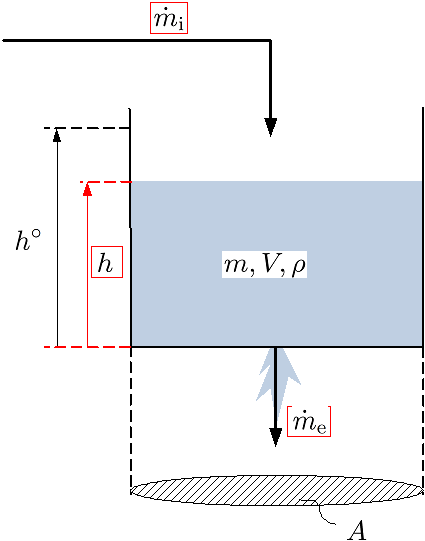
\includegraphics[width=\linewidth]{python_water_tank_model.png}
	\caption{Driven water tank, with externally available quantities framed	in red: initial mass is emptied through bottom at rate $\dot{m}_e $, while at the same time water enters the tank at rate $\dot{m}_i$ }
	\label{fig:pythonwatertankmodel}
\end{figure}

Our modeling objective is to find the liquid level h. This objective is illustrated by the functional diagram in
Figure \ref{fig:pythonwatertankfunctional}. The functional diagram depicts the causality of the system (“Tank with influent and effluent mass flow”), where inputs (green arrow) cause a change in the system and its output (orange arrow)\footnote{Although Modelica is an acausal modeling language, it is useful to think in terms of causality during model development.}. Here, the input variable is the influent mass flow rate $\dot{m}_i$, while the output variable is the quantity we are interested in, $h$.

\begin{figure}
	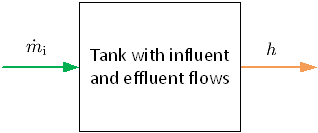
\includegraphics[width=\linewidth]{python_water_tank_functional.png}
	\caption{Functional diagram of tank with influent and effluent flow.}
	\label{fig:pythonwatertankfunctional}
\end{figure}

\subsection{Model Summary}
\label{subsec:pythonmodelsummary}

The model can be summarized in a form suitable for implementation in Modelica as:

\begin{equation*}
	\begin{aligned}
	    \frac{d_m}{d_t} = \dot{m}_i - \dot{m}_e \\
	     m = pV \\
	     V = Ah \\
	     \dot{m}_e = K\sqrt{\frac{h}{h^{\nabla^.}}} 
	\end{aligned}
\end{equation*}

To complete the model description, we need to specify model parameters and operating conditions. Model parameters
(constants) are given in Table \ref{tab:tablemodelparameters}, and the operating conditions are given in Table \ref{tab:tablemodeloperatingconditions}.

\begin{table}
	\begin{center}
		\caption{Parameters for driven tank with constant cross sectional area.} 
		\label{tab:tablemodelparameters} 
		\begin{tabular}{ cccc } 
			\hline
			\bfseries Parameter & \bfseries Value  & \bfseries Unit  & \bfseries Comment \\ 
			$p$ & $1$ & $kg/L $ & Density of liquid \\ 
			$A$ & $5$ & $dm^2$ & Constant cross sectional area \\ 
			$K$ & $5$ & $kg/s$ & Valve constant \\
			$h^{\nabla}$ & $3$ & $dm$ & Level scaling \\  
			\hline
		\end{tabular}
	\end{center}
\end{table}

\begin{table}
	\begin{center}
		\caption{Operating condition for driven tank with constant cross sectional area.} 
		\label{tab:tablemodeloperatingconditions} 
		\begin{tabular}{ cccc } 
			\hline
			\bfseries Quantity & \bfseries Value  & \bfseries Unit  & \bfseries Comment \\ 
			$h(0)$ & $1.5$ & $dm $ & Initial level \\ 
			$m(0)$ & $ph (0) A $ & $kg$ & Initial mass \\ 
			$\dot{m}_i (t)$ & $2$ & $kg/s$ & Nominal influent mass flow rate; may be varied \\
			\hline
		\end{tabular}
	\end{center}
\end{table}

\subsection{Water Tank Model expressed in Modelica}
\label{subsec:pythonmodleicamodel}

The Modelica code describes the core model of the tank, \textit{ModWaterTank}, and consists of a first section where
constants and variables are specified, and a second section where the model equations are specified.

\begin{lstlisting}
	model ModWaterTank 
		// Main driven water tank model 
		// author: Bernt Lie 
		// University College of 
		// Southeast Norway 
		// April 18, 2016 
		//
		// Parameters
		constant Real rho = 1 "Density";
		parameter Real A = 5 "Tank area";
		parameter Real K = 5 "Valve const";
		parameter Real h\_max = 3 "Scaling";
		// Initial state parameters
		parameter Real h\_0 = 1.5 "Init.level";
		parameter Real m\_0 = rho*h\_0*A "Init.mass";
		// Declaring variables
		// -- states
		Real m(start = m\_0, fixed = true) "Mass in tank, kg";
		// -- auxiliary variables
		Real V "Tank liquid volume, L";
		Real md\_e "Effluent mass flow";
		// -- input variables
		input Real md\_i "Influent mass flow";
		// -- output variables 
		output Real h "Tank liquid level,dm";
		// Equations constituting the model 
		equation 
		// Differential equation 
		der(m) = md\_i - md\_e; 
		// Algebraic equations 
		m = rho*V; 
		V = A*h;
		md\_e = K*sqrt(h/h\_max);
	end ModWaterTank;
\end{lstlisting}

As seen from the first section of model \textit{ModWaterTank}, the model has 4 essential parameters
$(rho-h_max)$, one of which is a Modelica constant $(rho)$ while the other 3 are design parameters (compare this
to Table I). Furthermore, the model contains 2 "initial state" parameters, where 1 of them can be chosen at
liberty, $h_0$, while the other one, $m_0$, is computed automatically from $h_0$, see Table II. The purpose of
the "free parameter" $h_0$ is that it is easier for the user to specify level than mass. Also, free "initial state"
parameters make it possible for the user to change the initial states from outside of model ModWaterTank, e.g., from Python.

Next, one variable is given with an initial value — the state $m$ — which is initialized with the "initial state" parameter
$m_0$. Then, 2 variables are defined as auxiliary variables (algebraic variables), $V$ and $md_e$\footnote{$md$ is notation for $m$ with a dot, $\dot{m}$ , i.e., a mass flow rate.}

One input variable is defined — $md_i$ — which is the influent mass flow rate $\dot{m}_i$, see Table \ref{tab:tablemodeloperatingconditions}. Inputs have the characteristic that their values are not specified in the core model — here\textit{ModWaterTank}. Instead,
their values must be given in an external model/code — we will specify this input in Python. Finally, 1 output is
given — $h$.

In the second section of model \textit{ModWaterTank}, the model equations exactly map the mathematical model
given in Section \ref{subsec:pythonmodelsummary}. For purposes of illustration, the core model \textit{ModWaterTank} is wrapped within a package named
\textit{WaterTank} and stored in file \textit{WaterTank.mo},


\begin{lstlisting}
	package WaterTank
		// Package for simulating
		// driven water tank
		// author: Bernt Lie
		// University College of
		// Southeast Norway
		// April 18, 2016
		//
		model ModWaterTank
		// Main driven water tank model
		// ....
		....
		end ModWaterTank;
		// End package
	end WaterTank;
\end{lstlisting}

\subsection{Use of Python API}
\label{subsec:pythonuseapi}

First, for example on Jupyter notebook, the following Python statements are executed:

\begin{lstlisting}
	from OMPython import ModelicaSystem
	import numpy as np
	import numpy.random as nr
	%matplotlib inline
	import matplotlib.pyplot as plt
	import pandas as pd
	LW = 2
\end{lstlisting}

Here, we use \textit{NumPy} to handle simulation results, etc. The random number package will be used in
a sensitivity/Monte Carlo study. The \textit{magic} function \textit{\%matplotlib inline} is used to embed Matplotlib
plots within the Jupyter notebook; to save these plots into files, simply right-click the plots. However, more options
for saving files are available if the magic function is \textit{excluded}, and the \textit{plt.show()} command is instead added
after the plot commands have been completed. The pandas library is used to illustrate presenting data in tables in a Jupyter
notebook. Finally, label \textit{LW} is used to give a conform line width in plots.

\subsection{Basic Simulation of Model}
\label{subsec:pythonsimulatemodel}

We instantiate object \textit{tank} by running the \acrshort{omc} Server with the following command:

\begin{lstlisting}
	tank = ModelicaSystem('WaterTank.mo','WaterTank.ModWaterTank')
\end{lstlisting}

Next, we are interested in which \textit{quantities} are available in the model. Python prompt \textit{>>>} is used when Jupyter
notebook actually uses \textit{In[*]} — where \textit{*} is some number, while the response in Jupyter notebook is prepended
with \textit{Out[*]}.

\begin{lstlisting}
	>>> q = tank.getQuantities()
	>>> type(q)
	list
	>>> len(q)
	11
	>>> q[0]
	{'Changeable': 'true', 
	'Description': 'Mass in tank, kg',
	'Name': 'm',
	'Value': None,
	'Variability': 'continuous'}
	>>> pd.DataFrame(q)
\end{lstlisting}

The last command leads Jupyter notebook to typeset a tabular presentation of the quantities, Figure \ref{fig:pythontypesetting}. The results
in Figure \ref{fig:pythontypesetting} should be compared to the Modelica model in \ref{subsec:pythonmodleicamodel}. Observe that Modelica \textit{constants} are not included in the quantity list.

\begin{figure}
	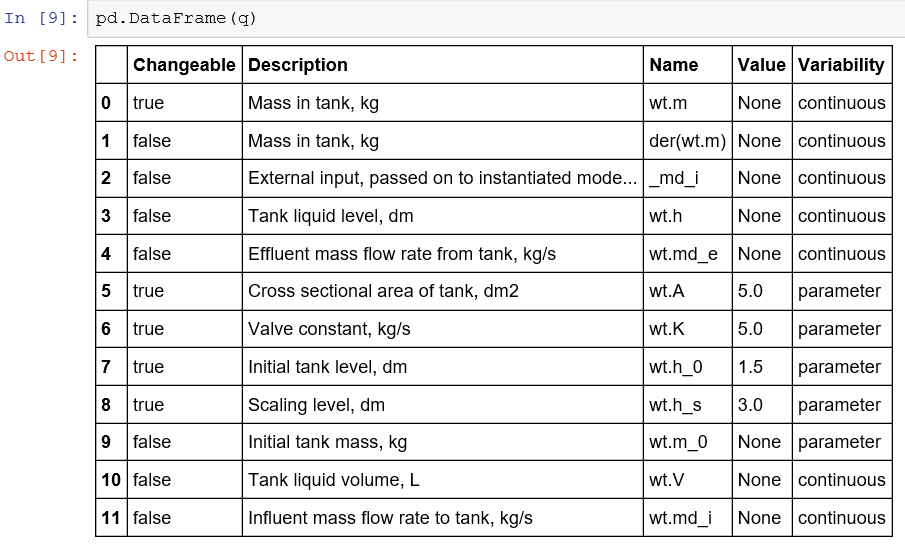
\includegraphics[width=\linewidth]{python_typesetting.png}
	\caption{Typesetting of Data Frame of quantity list in Jupyter notebook.}
	\label{fig:pythontypesetting}
\end{figure}

Next, we check the simulation options:

\begin{lstlisting}
	>>> tank.getSimulationOptions()
	{'solver': 'dassl',
	'startTime': 0.0,
	'stepSize': 0.002,
	'stopTime': 1.0,
	'tolerance': 1e-06}
\end{lstlisting}

It should be observed that the \textit{stepSize} is the frequency at which solutions are stored, and is not the step
size of the solver. The number of data points \textit{stored} is thus \textit{(stopTime-startTime)/stepSize} with appropriate
rounding. This means that if we increase the \textit{stopTime} to a large number, we should also increase the \textit{stepSize} to
avoid storing a large volume of information.


To this end, we want to simulate the system for a long time, until the level reaches a steady state. Possible inputs are:

\begin{lstlisting}
	>>> tank.getInputs(){'md_i': None}
\end{lstlisting}

where value None implies that the available input, $md_i$, has not yet been set. We could use \textit{None} as input, which will be interpreted as zero. 
But let us instead set $\dot{m}_i = 3$, simulate for a long time, and change the "initial state"
parameter $h (0)$ to the steady state value of $h$:

\begin{lstlisting}
	>>> tank.setInputs(md_i=3)
	>>> tank.setSimulationOptions\
	(stopTime=1e4, stepSize=10)
	>>> tank.simulate()
	>>> h = tank.getSolutions('h')
	>>> tank.setParameters(h_0 = h[-1])
\end{lstlisting}

Next, we set back the stop time to 10, and specify an input sequence with a couple of jumps:

\begin{lstlisting}
	>>> tank.setSimulationOptions\(stopTime=10, stepSize=0.02)
	>>> tank.setInputs(md_i = [(0,3),(2,3),(2,4),(6,4),(6,2),(10,2)])
\end{lstlisting}

Finally, we simulate the model with the time varying input, and plot the result:

\begin{lstlisting}
	>>> tank.simulate()
	>>> tm, h = tank.getSolutions('time','h')
	>>> plt.plot(tm,h,linewidth=LW,color='blue', label=r'$h$')
	>>> plt.title('Water tank level')
	>>> plt.xlabel(r'time $t$ [s]')
	>>> plt.ylabel(r'$h$ [dm]')
\end{lstlisting}

The result is displayed in Figure \ref{fig:pythonwatertanklevelplot}.

\begin{figure}
	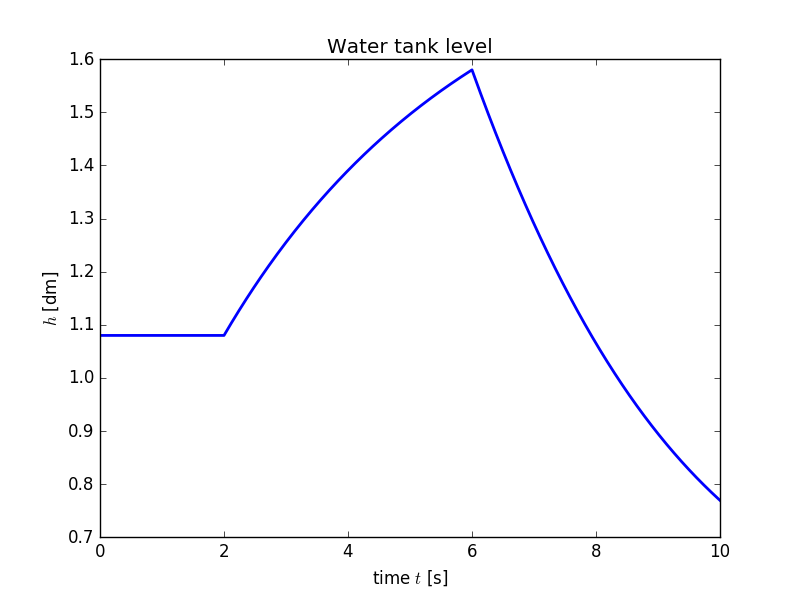
\includegraphics[width=\linewidth]{python_water_tank_level_plot.png}
	\caption{Tank level when starting from steady state, and $\dot{m}_i(t)$ varies in a straight line between the points $(tj,\dot{m}_i(t_j ))$
		given by the list $[(0; 3); (2; 3); (2; 4); (6; 4); (6; 2); (10; 2)]$.}
	\label{fig:pythonwatertanklevelplot}
	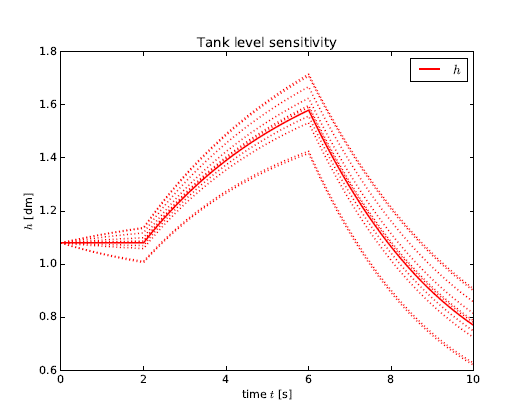
\includegraphics[width=\linewidth]{python_water_tank_level_sensitivity_plot.png}
	\caption{Uncertainty in tank level with a 5\% uncertainty in valve constant $K$. The input is the same as in Figure \ref{fig:pythonwatertanklevelplot}}
	\label{fig:pythonwatertanklevelsensitivityplot}
\end{figure}

\subsection{Parameter Sensitivity/Monte Carlo Simulation}
\label{subsec:pythonparametersensitivity}

It is of interest to study how the model behavior varies with varying uncertain parameter values, e.g., the effluent
valve constant $K$. This can be done as follows:

\begin{lstlisting}
	>>> par = tank.getParameters()
	>>> K = par['K']
	>>> KK = K + (nr.randn(10)-0.5)*K/20
	>>> tank.simulate()
	>>> tm, h = tank.getSolutions('time','h')
	>>> plt.plot(tm,h,linewidth = LW,color = 'red', label=r'$h$')
	>>> for k in KK:
		tank.setParameters(K=k);
		tank.simulate()
		tm, h = tank.getSolutions('time','h')
		plt.plot(tm,h,linewidth=LW,
		color='red',linestyle='dotted',label='_nolabel_')
	>>> plt.title('Tank level sensitivity')
	>>> plt.xlabel(r'time $t$ [s]')
	>>> plt.ylabel(r'$h$ [dm]')
	>>> plt.legend()
\end{lstlisting}

The result is shown in Figure \ref{fig:pythonwatertanklevelsensitivityplot}.

\section{Integration of Wolfram SystemModeler Simulator in PySimulator}
\label{sec:pythonwolframplugin}

PySimulator supports simulation of models in FMU form or using different Modelica tools via extension
plugins. Simulator plugins for tools such as Dymola, SimulationX, and OpenModelica are available from previous work. 
This section presents a new simulator plugin developed for Wolfram SystemModeler.

\begin{figure}
	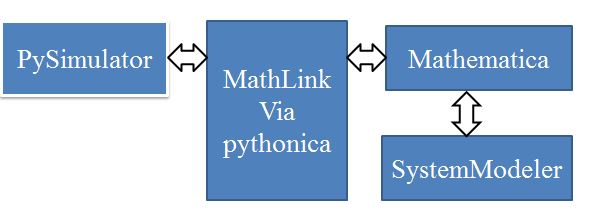
\includegraphics[width=\linewidth]{python_wolfram_communication.png}
	\caption{Communication setup with SystemModeler.}
	\label{fig:pythonwolframcommunication}
\end{figure}

Wolfram SystemModeler has its own symbolic mathematical computation program, Mathematica \cite{mathematica}, which can be used
to perform actions via the Wolfram SystemModeler link (WSMLink) API \cite{wsmlink}, such as loading, compilation and 
simulation of models, or plotting of results. WSMLink provides functionality for integrating Wolfram SystemModeler and Mathematica  
with complete access to models and simulations.

Wolfram SystemModeler can be interfaced to other tools via MathLink \cite{mathlink}, which is a library of functions that 
implement a protocol for sending and receiving Mathematica expressions. MathLink \cite{mathlinktutorial,mathlink} allows external
programs to both call Mathematica and be called by Mathematica. It is possible to create a front end that 
implements your own user interface and communicates with the Mathematica kernel via MathLink \cite{mathlinkc}.

Using the existing interface for simulator plugins in PySimulator, a new simulator plugin has
been implemented: the Wolfram plugin. It enables PySimulator to load and numerically simulate
Modelica models using Wolfram SystemModeler.

The Wolfram plugin is integrated into PySimulator via MathLink and Pythonica \cite{pythonica}, which connects to Mathematica and
SystemModeler. We used the Wolfram SystemModeler API to support loading a Modelica model, simulating
it, and reading the simulation setting file (\textit{.sim}), which is an XML file, to build the variable tree in the
variables browser of PySimulator. The overall communication setup with SystemModeler is given in
Figure \ref{fig:pythonwolframcommunication}.

All of the simulator plugins of PySimulator are controlled by the same Integrator Control GUI. The Wolfram
SystemModeler simulator supports five different numerical integration methods (\textit{DASSL, CVODES,
Euler, RungeKutta, and Heun}), all the simulation menu options are supported (\textit{error tolerance, fixed step
size}, etc.), see Figure \ref{fig:pythonintegratorcontrol}.

\begin{figure}
	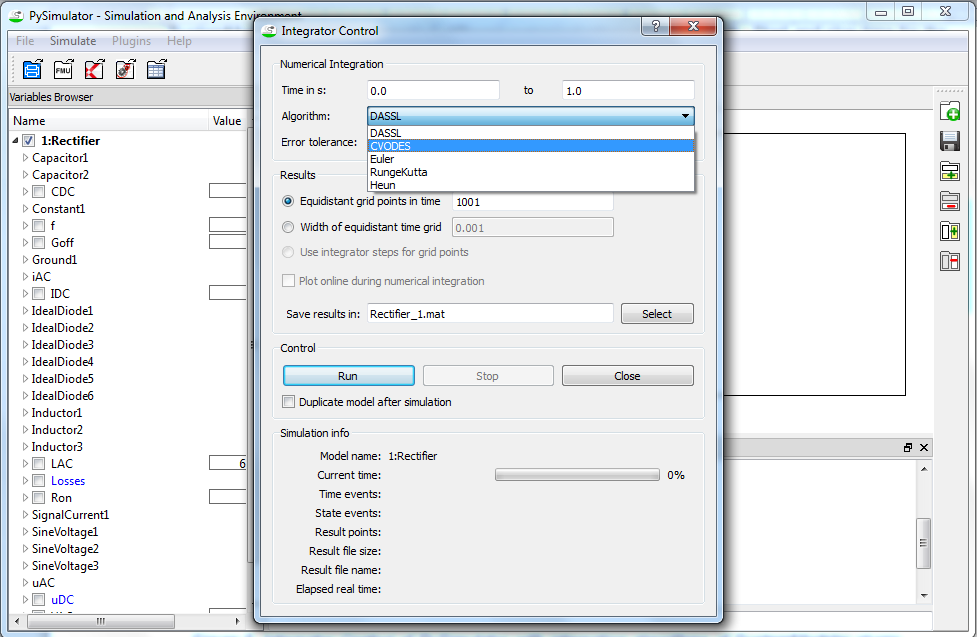
\includegraphics[width=\linewidth]{python_integrator_control.png}
	\caption{Integrator Control of PySimulator with integration algorithms of SystemModeler plugin.}
	\label{fig:pythonintegratorcontrol}
\end{figure}

The \textit{start} and \textit{stop time} for the integration algorithm can be changed and one of the integration algorithms
can be selected. Depending on the integration algorithms the user can change the \textit{error tolerance} or the \textit{fixed step size}
before running the simulation.

It is also possible to simulate the list of models using the Wolfram plugin. The existing PySimulator interface automatically 
includes the new plugin in the simulators list for simulating a list of models.

\begin{landscape}
\begin{figure}
	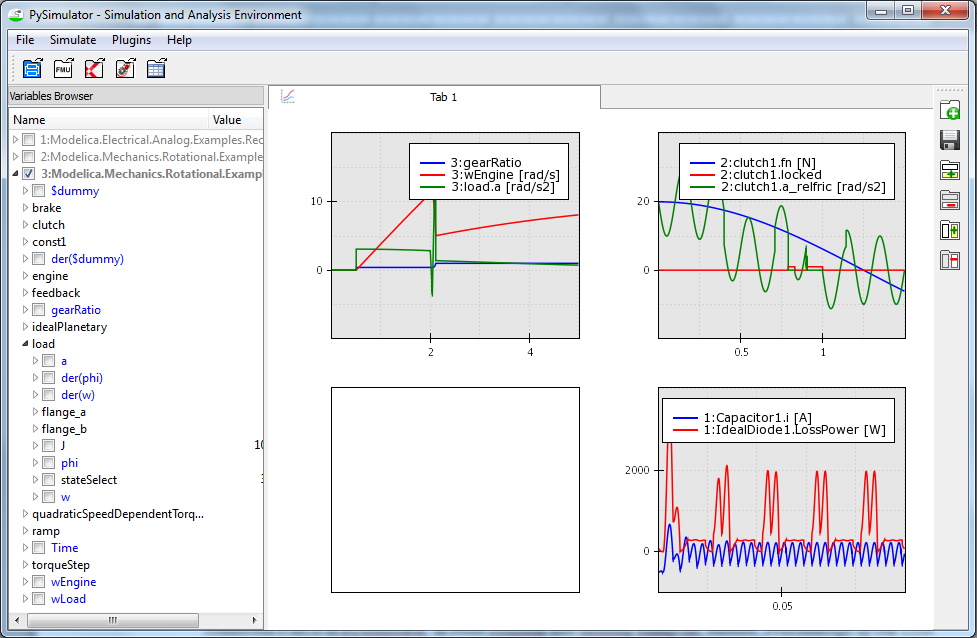
\includegraphics[width=\linewidth]{python_list_of_simulate_models.png}
	\caption{List of simulate models via Wolfram plugin.}
	\label{fig:pythonlistofsimulatemodels}
\end{figure}
\end{landscape}

\section{Summary}
\label{sec:pythonsummary}

In this chapter, we have introduced an enhanced Python interface for interacting with FMUs and Modelica models for further analysis and post-processing of simulation results. We have presented how a modeler can use the Python interface to simulate and access Modelica models using Python objects. The idea behind this interface is to provide the modeler with the ability to manipulate and exchange data with Modelica models before and after simulations. A case study of a Modelica model is presented to illustrate the tool’s usage.

We have also presented a simulator plugin for a commercial simulation engine for Modelica models - the Wolfram SystemModeler within PySimulator. The existing PySimulator interface automatically includes the new plugin in the simulators list for simulating lists of models. We have successfully tested by loading all of the result files generated from the Wolfram plugin and verified the results by comparing with several other base line tools. The integration of the Wolfram SystemModeler simulator plugin uses the regression analysis framework within PySimulator to compare results of the same model generated from SystemModeler with several other tools or different versions of the same model from the SystemModeler tool.

\subsection*{Acknowledgments}
\label{sec:pythonacknowledgments}

Part of the PySimulator work is financed by the CleanSky Joint Undertaking project PyModSimA (JTI-CS-2013-2-
SGO-02-064). This support is highly appreciated. The authors thank Jakub Tobolar (DLR
Institute of System Dynamics and Control) for his tests and support of the regression testing feature in an
earlier stage and his implementation of the automatic generation of the simulation setup file by Dymola.

%\nocite{scigen}
%We have included Paper \ref{art:scigen}

%%%%%%%%%%%%%%%%%%%%%%%%%%%%%%%%%%%%%%%%%%%%%%%%%%%%%%%%%%%%%%%%%%%%%%
%%% Intro.tex ends here


%%% Local Variables: 
%%% mode: latex
%%% TeX-master: "demothesis"
%%% End: 


%%% lorem.tex --- 
%% 
%% Filename: lorem.tex
%% Description: 
%% Author: Ola Leifler
%% Maintainer: 
%% Created: Wed Nov 10 09:59:23 2010 (CET)
%% Version: $Id$
%% Version: 
%% Last-Updated: Wed Nov 10 09:59:47 2010 (CET)
%%           By: Ola Leifler
%%     Update #: 2
%% URL: 
%% Keywords: 
%% Compatibility: 
%% 
%%%%%%%%%%%%%%%%%%%%%%%%%%%%%%%%%%%%%%%%%%%%%%%%%%%%%%%%%%%%%%%%%%%%%%
%% 
%%% Commentary: 
%% 
%% 
%% 
%%%%%%%%%%%%%%%%%%%%%%%%%%%%%%%%%%%%%%%%%%%%%%%%%%%%%%%%%%%%%%%%%%%%%%
%% 
%%% Change log:
%% Completed Language Reading MBS
%% 
%% RCS $Log$
%%%%%%%%%%%%%%%%%%%%%%%%%%%%%%%%%%%%%%%%%%%%%%%%%%%%%%%%%%%%%%%%%%%%%%
%% 
%%% Code:

\chapter{Conclusions and Future Work}
\label{cha:conclusionsandfuturework}

\section{Conclusions}
\label{sec:conclusions}

The main goal of this thesis was to design and implement tools and methods, up to the point of proof of concept and prototype demonstrations, which would increase the efficiency and quality of model-based development of complex and multi-domain cyber-physical systems.

With respect to the objective “to ensure automatic solution of dynamic optimization problems by reusing simulation models for optimization”, we have developed a model-based dynamic optimization approach by integrating optimization into the model development process. The feasibility of our approach was demonstrated by a prototype implementation that was employed in the solution of industrially-relevant optimal control problems, including a diesel engine model. While the parameter sweep static design optimization method uses many simulation runs, the dynamic optimization approach presented in this thesis uses a direct optimization of a whole solution trajectory iteratively to obtain the optimal solution with minimum computation and time. OpenModelica coupling with CasADi has shown that it’s possible to use an XML-based model exchange format for model-based dynamic optimization with state of the art optimization algorithms. The approach contributes to enabling mathematical simulation models expressed in Modelica with the Optimica language extension to be used efficiently for simulation-based optimization. The use of a language-neutral model exchange format simplifies tool interoperability and allows modelers to conduct experiments with different optimization algorithms and choose the one that is best suited for their particular problem, without the need to re-encode the problem formulation. As compared to traditional optimization frameworks, which typically require modelers to encode the model, the cost function, and the constraints in an algorithm-specific manner, the approach presented in this thesis significantly increases flexibility.  

With respect to the objective “to ensure reusing and combining existing simulation models formalized by different experts in different modeling languages and tools for a unified system simulation”, we have developed a general open-source graphical and textual editor, and a co-simulation framework for composite modeling and simulation of several connected subsystems using detailed models. Several tool-specific simulation sub-models can be integrated and connected by means of a composite model, represented in XML, which defines the physical interconnections between them. The approach is based on a general external interface definition that can be implemented for many different simulation tools using the TLM method. This enables de-coupling of sub-models from the full system and allows them to be independently simulated and coupled in a numerically stable way via co-simulation techniques. Currently, most simulation tools for model-based development of cyber-physical systems are bound to a specific tool vendor. An open-source modeling and co-simulation environment for composite models will change that, since it enables integration of models defined in a specific language from many different simulation tool vendors in the design process. It has been successfully implemented and tested for several simulation tools. 

With respect to the objective “to support advanced simulation modeling analysis”, we have enhanced the Python interface to simulate and access EOO Modelica models using Python objects for further simulation modeling analysis. Our tool, OMPython, is developed as a library using a standard distribution of Python and targeted to the OpenModelica modeling and simulation environment. However, general concepts can be applied to any other language and tool. In order to ensure reusability, only the standard Python libraries were used. From a modeler’s perspective, the Python interface makes scripting, plotting, and analysis of results straightforward. This gives the modeler the possibility to use EOO simulation models together with the more powerful and easier to use API and Python libraries, e.g., for tasks such as control design and post processing of simulation results. 

We have also extended the list of simulator plugins for PySimulator by implementing a plugin for Wolfram’s SystemModeler. The integration of Wolfram SystemModeler simulator plugin uses the simulation result analysis tools within PySimulator. Hence, comparing simulation results of the same model generated from SystemModeler with several other tools or different versions of the same model from the SystemModeler tool can be applied. Comparing results of model simulations is very important for model portability and model evolution. This makes it possible for simulation models from SystemModeler to be safely utilized and integrated into different tools in the design process.

With respect to the objective “to ensure automatic traceability between requirements, simulation models, FMUs, and simulation results artifacts and keep track of changes and integration of product design tools with modeling and simulation tools”, we have developed a tool-supported method for multi-domain collaborative modeling and traceability support throughout the developments in CPSs. A design and implementation for seamless tracing and interoperability of lifecycle artifacts in OpenModelica, integrated with the INTO-CPS tool-chain of CPS design, has been developed based on a linked data approach. A tool interoperability approach based on the Linked data method for traceability improves the reusability of simulation models between tools in distributed collaborative development flows. Hence, system designers and analysts with expertise in different domains can effectively collaborate on the design of complex systems. The approach presented in this thesis contributes to an important step in the integration of different modeling tools that are used in the whole tool-chain of CPS design, from systems modeling down to co-simulation and test automation. This can be used to support several activities such as impact analysis, component reuse, verification, and validation. 

The message format and schema for the traceability information has been standardized in order to ensure that all tools use the same format for sending their trace data. This schema, together with the use of standardized specifications and formats, allows other tool vendors to easily integrate their tools into the INTO-CPS tool-chain traceability environment. Currently, the traceability data is stored in a graph database that can be queried in order to generate various reports, such as impact analysis. Furthermore, users can easily query this database to retrieve specific information about the links between different entities, such as requirements, users, test results or models (FMUs).

\section{Future Work}
\label{sec:futurework}

Seamless traceability throughout the development life cycle, such as from the design model to simulation results, for CPSs are active research areas. 
Our work on traceability came about through integration with the INTO-CPS tool-chain of CPS design. 
It is our intention to explore seamless tracing of the requirements and associating them with the models and the simulation results 
in the same language and with a single tool. This reduces the semantic gap in the terminology used between the requirement verification engineers and 
the system modelers, which in turn simplifies the modeling effort and allows for automated combination between the requirement models.
For impact analysis, we would like to develop queries over the traceability data starting from requirement verification reports.
Ultimately, we plan to conduct larger industrial use case to assess the extent to which system modelers benefit from our framework.

%%%%%%%%%%%%%%%%%%%%%%%%%%%%%%%%%%%%%%%%%%%%%%%%%%%%%%%%%%%%%%%%%%%%%%
%%% lorem.tex ends here

%%% Local Variables: 
%%% mode: latex
%%% TeX-master: "demothesis"
%%% End: 




% And print the references (by default in references.bib)
\printbibliography

% Demonstrates the use of included publications, for graduate-level theses
% \includearticle{scigen}
% \includearticletex{scigen}

\end{document}

%%%%%%%%%%%%%%%%%%%%%%%%%%%%%%%%%%%%%%%%%%%%%%%%%%%%%%%%%%%%%%%%%%%%%%
%%% demothesis.tex ends here

